% !TEX root = ../thesis_main.tex



%%%% --- * --- %%%%
\clearpage	
%\chapter{Estimating Systematic Effects}
\chapter{Analysis and Estimates of Systematic Effects}
\label{systematics_chapter}
\label{analysis_chapter} 
\note{Go through and change all instances of ``Beta - SOE''/``Beta---SOE''/etc to ``SOE -  Beta''/etc., *within the whole thesis*.}
%I really need an excuse to include more pictures of data.  Also, more pictures of simulations.
%\missingfigure{Show simulated spectra separated by scattering category.}
%\note[color=tag]{Re-phrase (or at least un-pinken) Analysis Chapter intro blurb from John.}
\note[color=jb]{John proposes the following intro statement for this Ch.~\ref{analysis_chapter} The following two(one) paragraphs are (almost) a direct quote from him:  }
%\note[color=jb]{JB:  Here is what I suggest for the intro the Analysis section:  (n.b.:  at the time of this comment, that was Ch.7)
%\\...\\
%7.0
%\comment{
%\\...\\

The collaboration has performed an independent analysis using (mostly) the same set of data to measure $\Abeta$, fixing $\bFierz$ to zero.
Differences with that analysis are interleaved in this section~\aside{Are they even though??} and summarized in Appendix~\ref{ch:differences_data}.
Critical physics improvements concern an eMCP-beta timing walk correction which enabled an improved cut against background, also incorporating a more complete modelling of decay backgrounds from untrapped atoms. Technical corrections include a correct treatment of the polarization cycle.
An arbitrary change in the DSSD
%deltaE 
radius cut is kept self-consistent.
%}


%\note[color=jb]{JB:  ``I doubt I will have further useful comments on the Ch. (((this chapter))) as they are now.}
\note[color=jb]{JB:  \\
I've tried to email you the paragraphs on "collaboration determination of uncertainties" for (((Ch.~\ref{systematics_chapter})))
\\
My intent of all that other advice  was to keep your time spent on Chs 1-4 ((Now Ch. 1-2)) concise, so you could concentrate on these real jobs.  (n.b.:  the advice he's already sent was almost all about chapters 1-4, which are the various intros/background info and experimental setup stuff)
\\ ... \\
I can only say that if you have an equal choice between including a detail or not, pick "not." ''
}
%\note[color=jb]{JB:  I will try to schedule meeting with Dan for you to show us the final version of (((Ch.~\ref{systematics_chapter}))) Estimating systematic effects soon.}

%\note[color=org]{Do I want this chapter combined with the analysis chapter?  If that chapter includes all the stuff about G4, it's going to be unwieldy and huge.}
%\note{How do I even \emph{do} these estimations?}

%%%%\note[color=todoblue]{JB says:   
%%%%\\
%%%%A simple estimate from the collaboration that builds intuition for this result:
%%%%Scatter in the SiC mirrors and DSSD actually produces an efficiency change at low
%%%%beta energy. Energy loss is not minimally ionizing in these structures, and instead
%%%%will have a long Landau tail that can take events below energy threshold in the scintillator.
%%%%The collaboration has modelled explicitly the false asymmetry as a function
%%%%of Kbeta between 600 and 1300 keV, producing roughly (K-0.6 MeV)/(0.7 MeV), i.e.
%%%%50\% at Kbeta=0.95 MeV. This efficiency degradation would be distributed roughly equally
%%%%between the SiC and DSSD.
%%%%If completely ignored, this would introduce by inspection a false bFierz of approximately
%%%%0.5.
%%%%Scattering effects will vary between linear and sqrt of thickness, so assuming
%%%%worst case of linear, the mechanical thickness uncertainty
%%%%of 5 micron/300 micron and 6 micron /275 micron, an average of 2\%, making
%%%%a random contribution of order 0.01 each.
%%%%The Be window has larger mechanical thickness uncertainty of 23micron/229 micron, but
%%%%energy loss and scattering in this material is 5x smaller, so the net effect would be similar.
%%%%\\ ... \\
%%%%To minimize this systematic for future experiments, the collaboration has
%%%%implemented pellicle mirrors of negligible thickness, 100 nm Au on 4 micron
%%%%kapton. The collaboration is also implementing Be-windowed wire chambers in
%%%%place of the DSSD.
%%%%\\
%%%%...
%%%%\\
%%%%MJA:  .....huh?
%%%%}
%%%%


%%%% --- * --- %%%%
%%%% --- * --- %%%%
\FloatBarrier
\section{Comparing Simulations to Experimental Data:  The General Methodology}
\label{sec:comparing_data_sims}
The primary parameter measurement strategy in this project involved comparing the experimental data to a 2D parameter space of simulations, and this is true both for evaluation of the best parameter values, and also for evaluations of the uncertainties.  

As described in Section~\ref{signature_chapter}, and in more detail in Appendix~\ref{appendix:superratio}, the primary experimental observable is the superratio asymmetry, which is constructed from four experimental \emph{rates} of beta detection:
\bea
A_{\mathrm{super}}(\Ebeta) 
&=& 
\frac{ \sqrt{r_{\mathrm T-}\, r_{\mathrm B+} \phantom{ (\!\!\!\!\!) } }\; -\, \sqrt{ r_{\mathrm T+}\, r_{\mathrm B-}\phantom{ (\!\!\!\!\!) }} }{ \sqrt{r_{\mathrm T-}\, r_{\mathrm B+}\phantom{ (\!\!\!\!\!) }} \;+\, \sqrt{r_{\mathrm T+}\, r_{\mathrm B-} \phantom{ (\!\!\!\!\!) }} }.
\eea
This quantity is closely related to the two fundamental parameters we hope to extract, 
%$\Abeta$ and $\bFierz$, 
and in the absence of certain systematic effects, we can cleanly describe a relationship between the observable
%, $A_{\mathrm{super}}(\Ebeta)$, 
and the two physical parameters ($\Abeta$ and $\bFierz$) that we might use to describe the shape of an experimentally measured $A_{\mathrm{super}}(\Ebeta)$ curve:
\bea
A_{\mathrm{super}}(\Ebeta) 
&=&
%&\approx& 
\frac{\Abeta \, \frac{v}{c} \, |\vec{P}| \, \langle | \cos\theta | \rangle
}{
1 + \bFierz \frac{mc^2}{\Ebeta}
}.
\label{eq:AsuperAbetabFierz}
\eea

Of course, when all systematics are properly accounted for, Eq.~\ref{eq:AsuperAbetabFierz} is no longer an adequate description of the full relationship between the observable and physical parameters and a comparison to monte carlo must be used.  A series of Geant4 simulations are performed and the results are (re-)processed with slightly different cuts and calibrations so as to match with the experimental conditions in each of the three electron datasets, and the superratio asymmetries are constructed.  The degree to which the simulations and experiment match is evaluated by using a $\chi^2$ comparison of the superratio asymmetries as the figure of merit (see Figs.~\ref{fig:asymmetryB},\ref{fig:asymmetryC},\ref{fig:asymmetryD}).  This is repeated for a range of $\Abeta$ and $\bFierz$ values, and a $\chi^2$ mapping of the 2D parameter space is produced.  

%
\begin{figure}[h!t!b!]
	\centering
	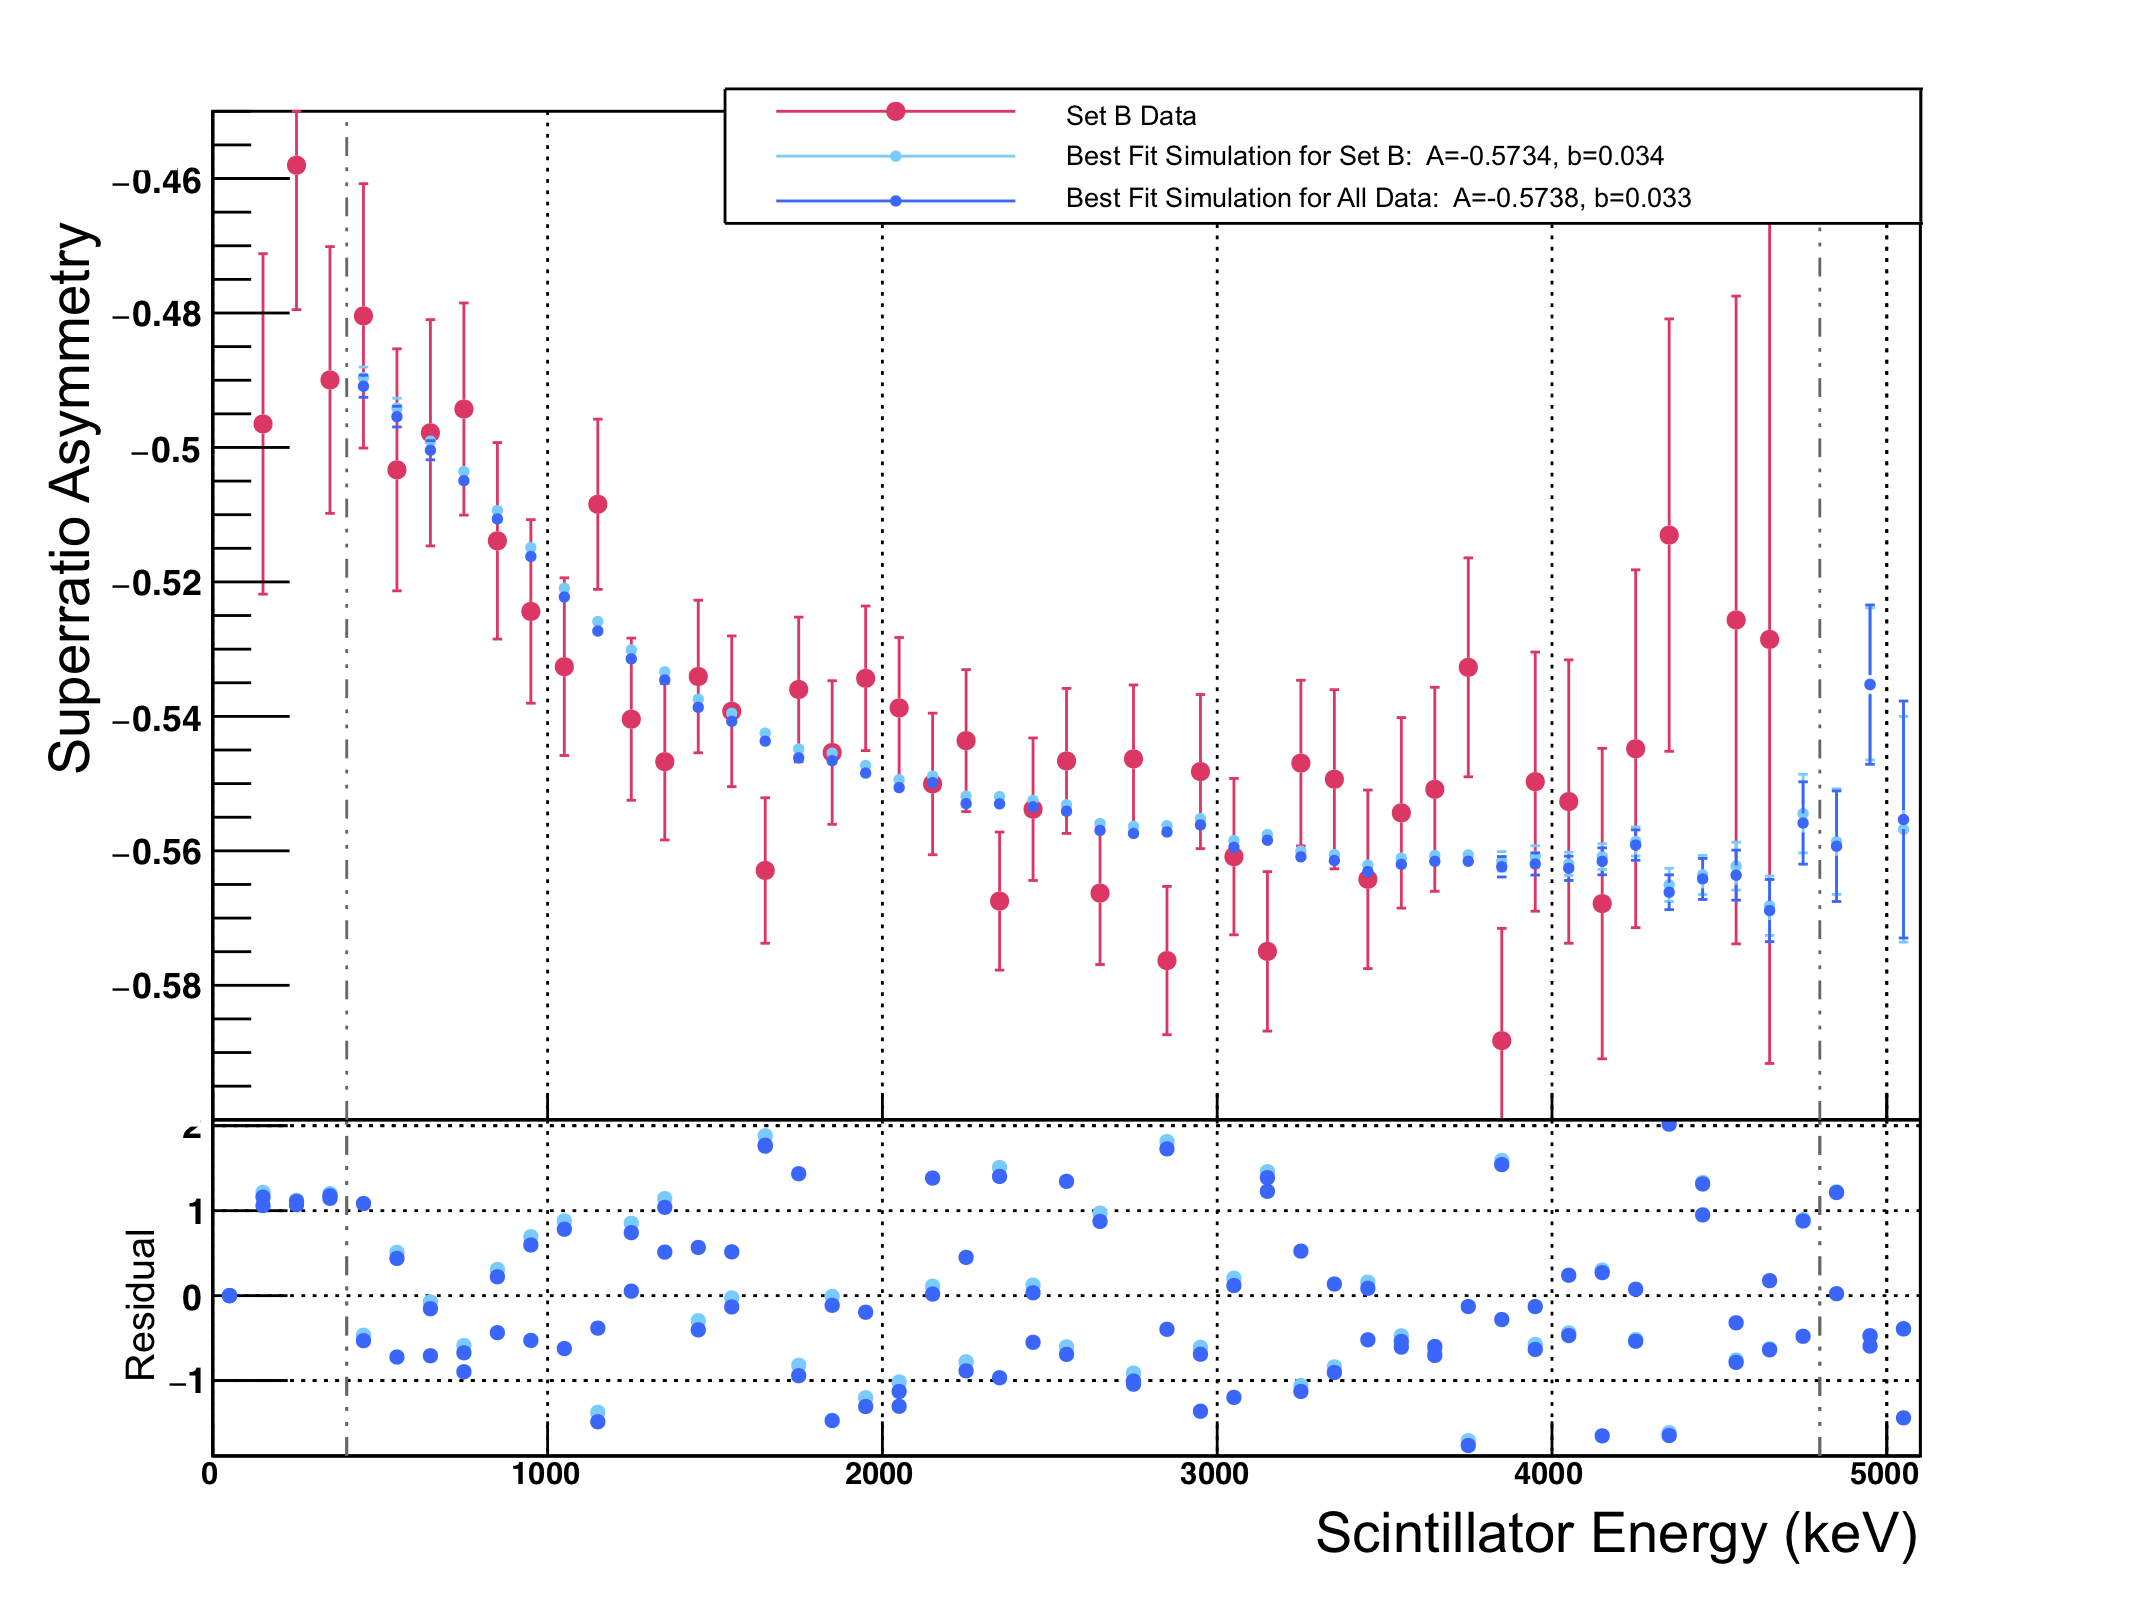
\includegraphics[width=.999\linewidth]
	{Figures/BestAsymmetry_SetB.png}
	\caption[SetB Superratio Asymmetry]{A superratio asymmetry from Dataset B, and the best fits from simulations.}	
	\label{fig:asymmetryB}
\end{figure}
%
\begin{figure}[h!t!b!]
	\centering
	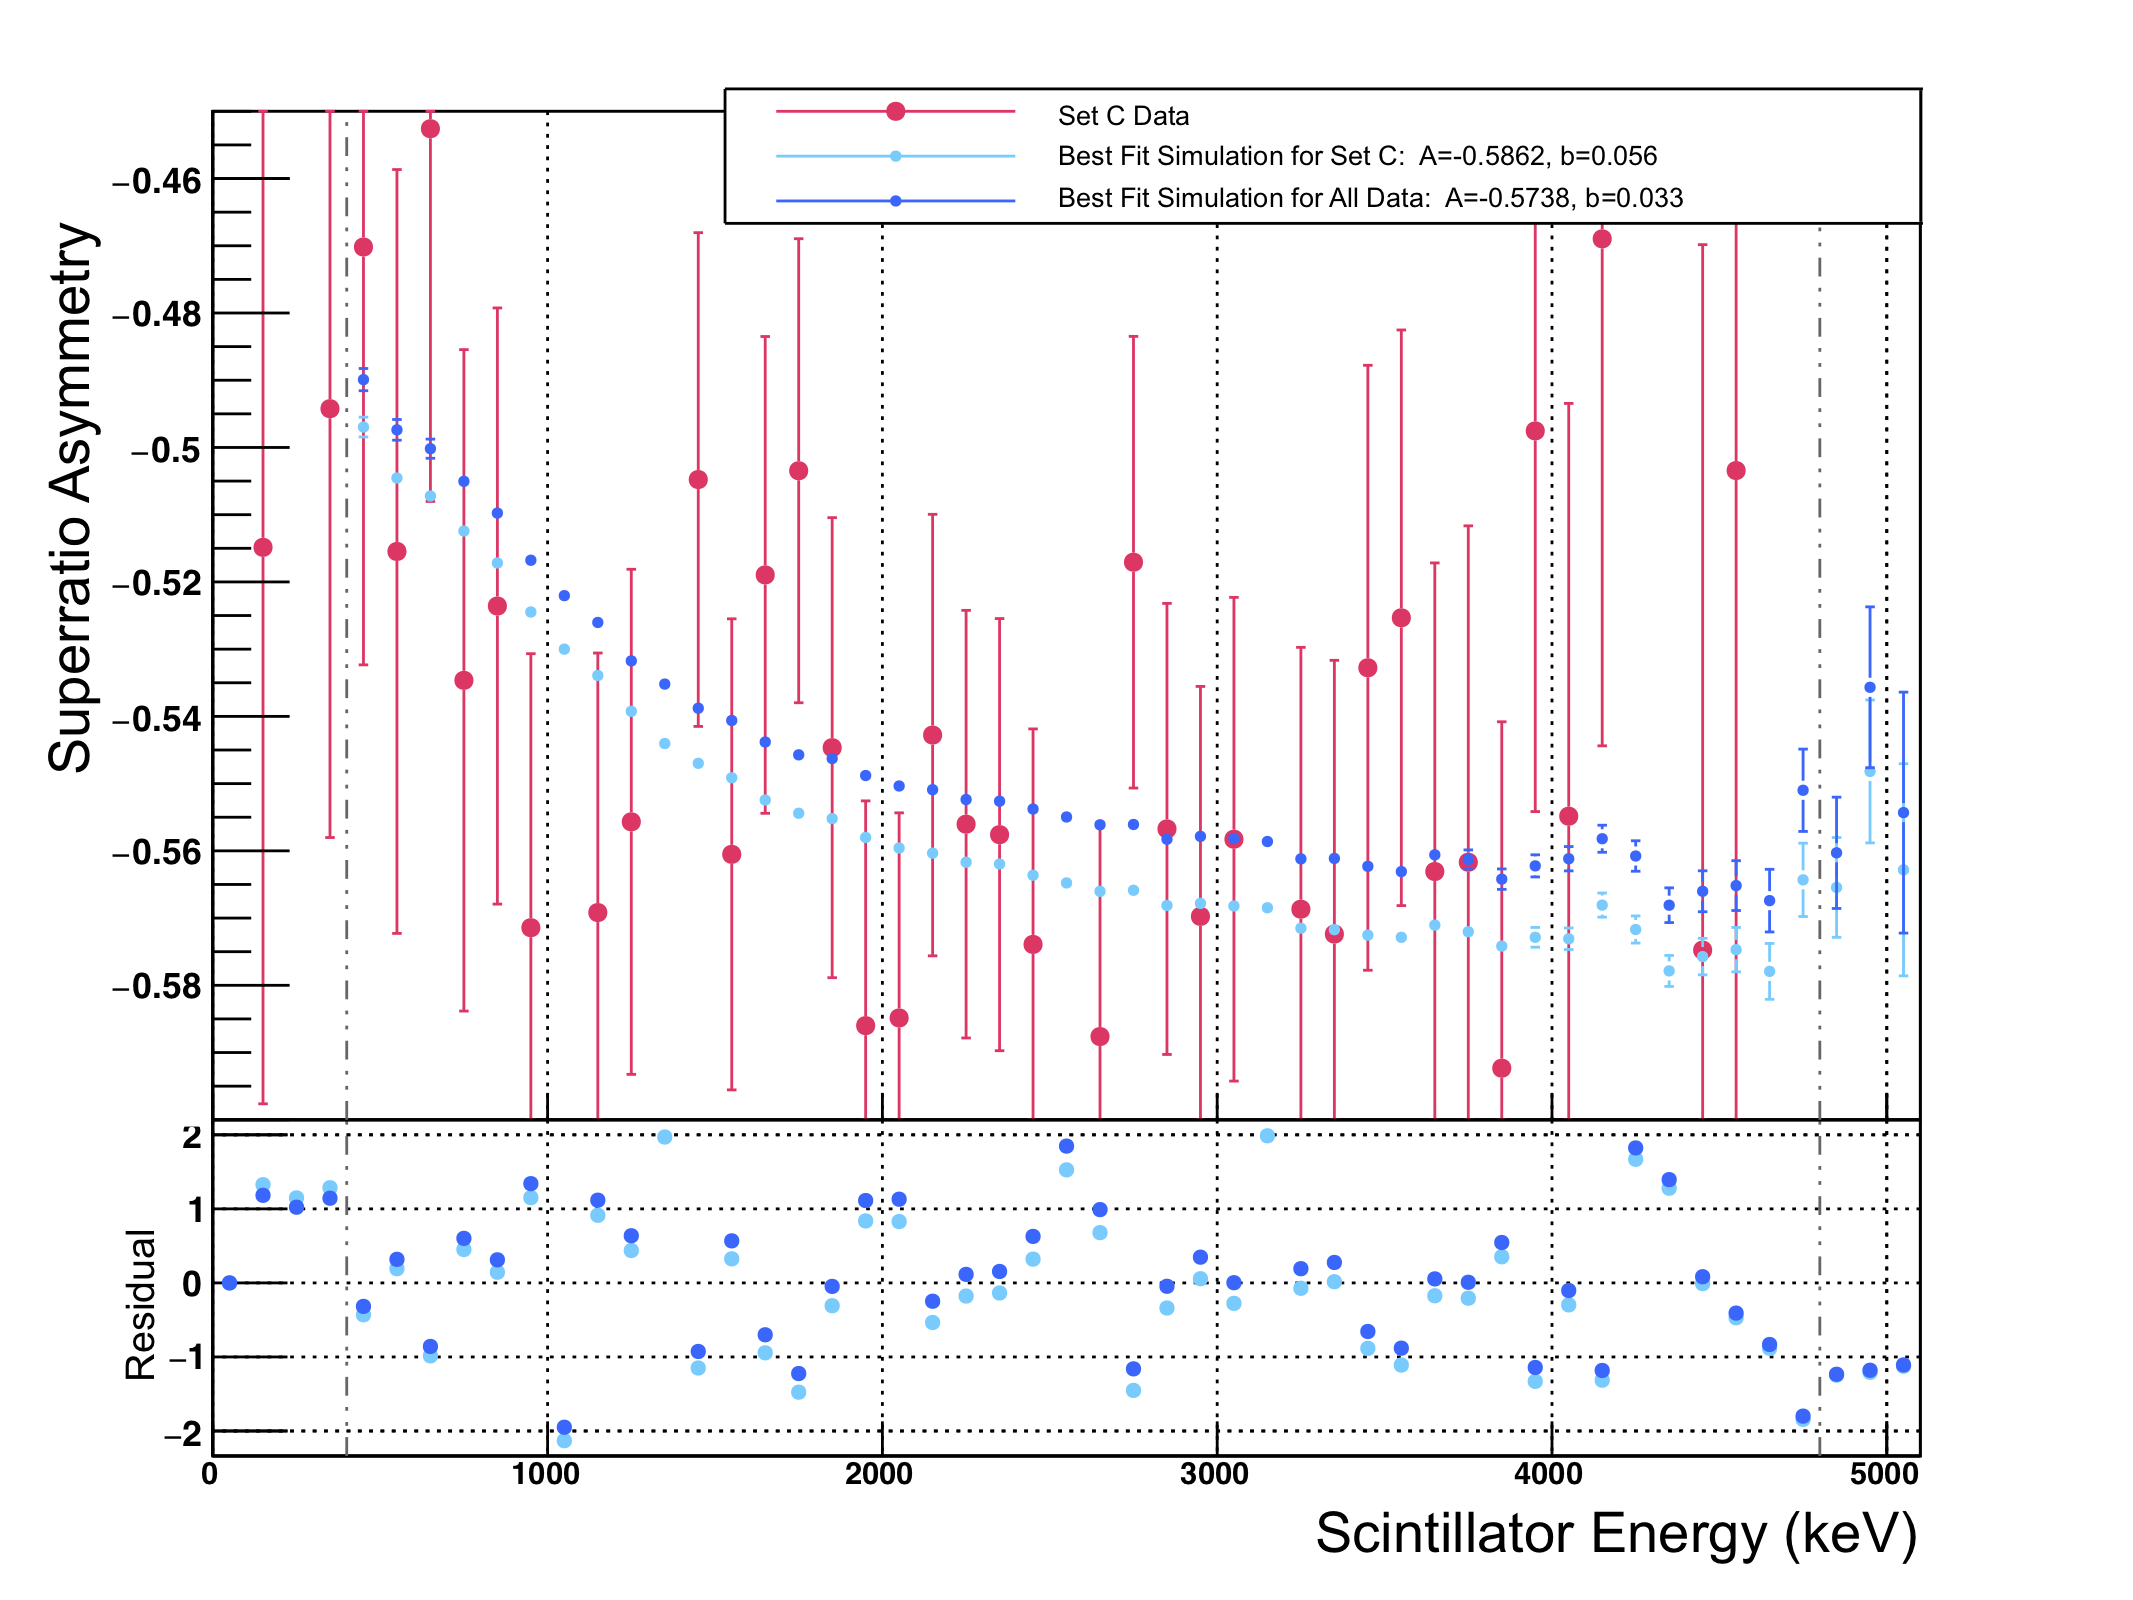
\includegraphics[width=.999\linewidth]
	{Figures/BestAsymmetry_SetC.png}
	\caption[SetC Superratio Asymmetry]{A superratio asymmetry from Dataset C, and the best fits from simulations.}	
	\label{fig:asymmetryC}
\end{figure}
%	
\begin{figure}[h!t!b!]
	\centering
	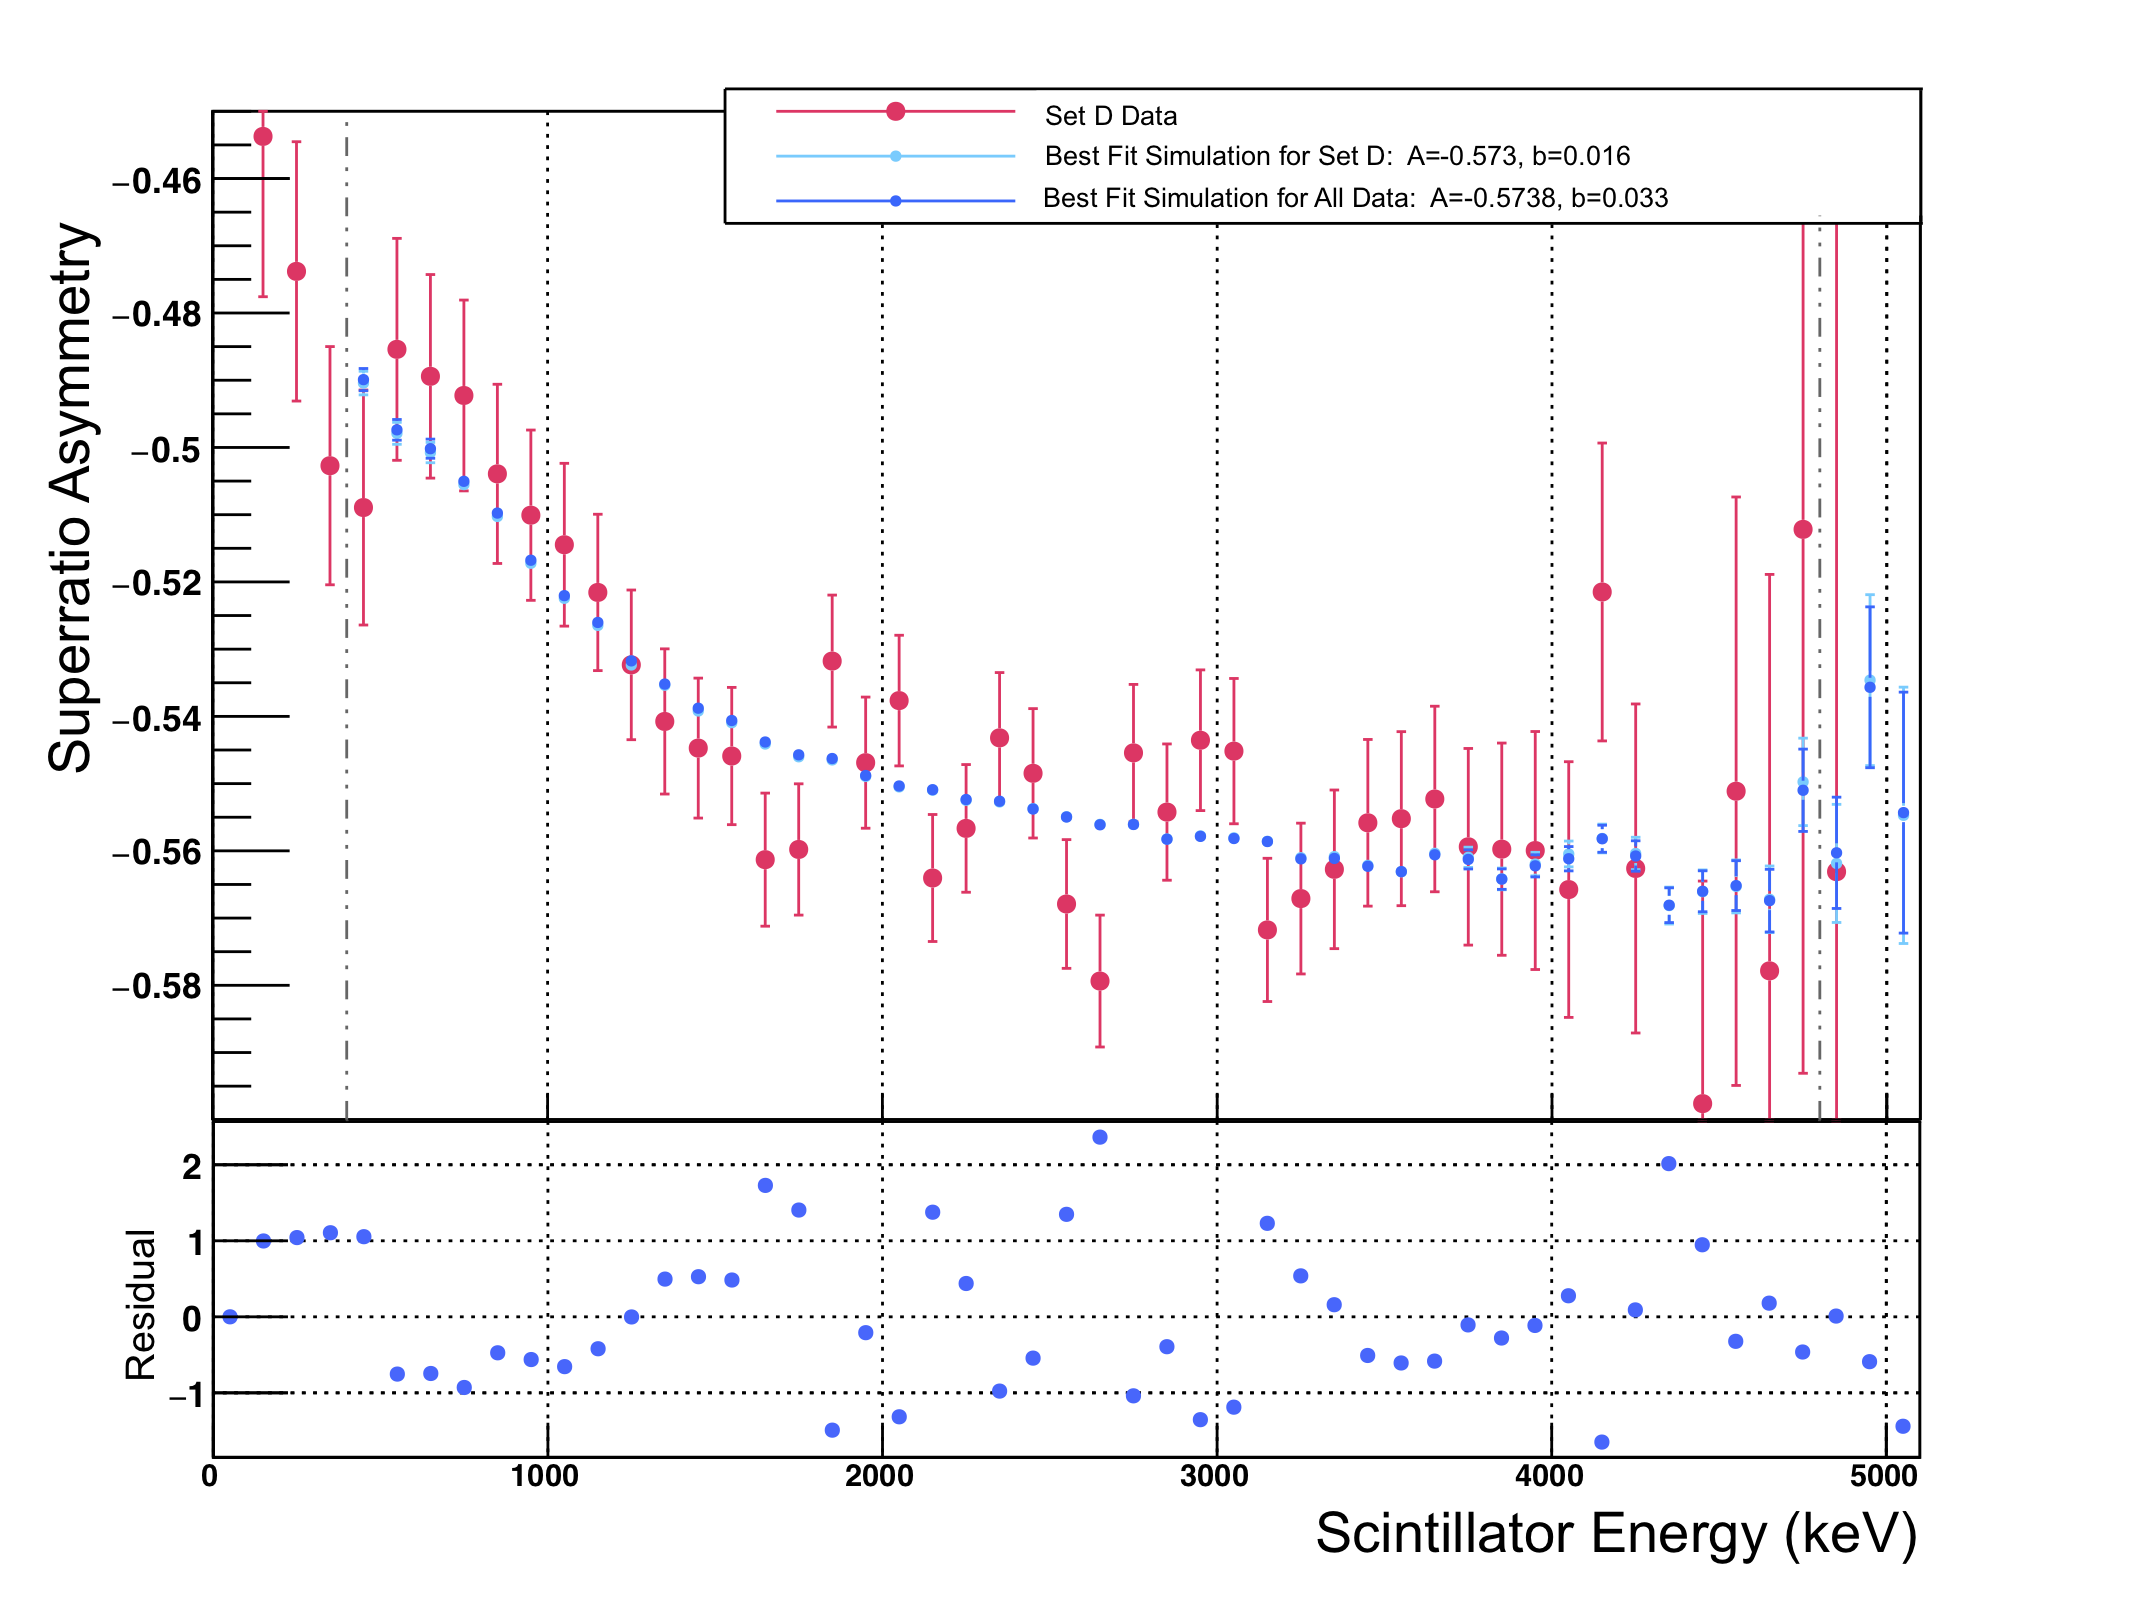
\includegraphics[width=.999\linewidth]
	{Figures/BestAsymmetry_SetD.png}
	\caption[SetD Superratio Asymmetry]{A superratio asymmetry from Dataset D, and the best fits from simulations.}	
	\label{fig:asymmetryD}
\end{figure}
%

For each superratio asymmetry constructed from simulated spectra, the scintillator spectra from which the superratio asymmetry is comprised are created as a linear combination of Geant4 beta decay events originating from the atom cloud and from surfaces within the chamber.  Both components of the spectra are combined event-by-event with SOE events generated in COMSOL, as described in Sections~\ref{sec:bs} and~\ref{sec:tof_bg}, as this is necessary for the critical time-of-flight cut on the ``SOE -- Beta'' spectra.  For decays originating within the atom cloud, both the primary decay branch and the subdominant `two percent' branch are allowed to contribute events, and only the dominant branch is varied as a function of BSM couplings.  For background events, only the Standard Model primary branch is simulated.  

A major caveat to the above description is that running a high statistics G4 simulation of our experiment is a computationally expensive process, so it was not possible to perform a separate simulation at every `pixel' within the parameter space.  Instead, to evaluate how well the experimental data matched to the expectation for varying values of $\Abeta$ and $\bFierz$, only three simulations were performed for different values of $\bFierz$, all using the same nominal value for $\Abeta$.  The $A_{\mathrm{super}}(\Ebeta)$ spectra representing intermediate $\bFierz$ values were created from a linear combination of spectra generated at the two closest values of $\bFierz$.

To vary the effective $\Abeta$ value, the generated $A_{\mathrm{super}}(\Ebeta)$ spectrum was simply scaled.  From Eq.~\ref{eq:AsuperAbetabFierz} it is clear that this works well so long as $\bFierz$ is small and any systematics are evaluated separately.  This method allows for an arbitrarily finely pixellated 2D $\chi^2$ map to be created.  It is done separately for each of the three experimental data sets so as to facilitate evaluation of systematic effects that changed between runsets.  See Figs.~\ref{fig:2dchi2_setB},\ref{fig:2dchi2_setC},\ref{fig:2dchi2_setD}.

\begin{figure}[h!tb]
	\centering
	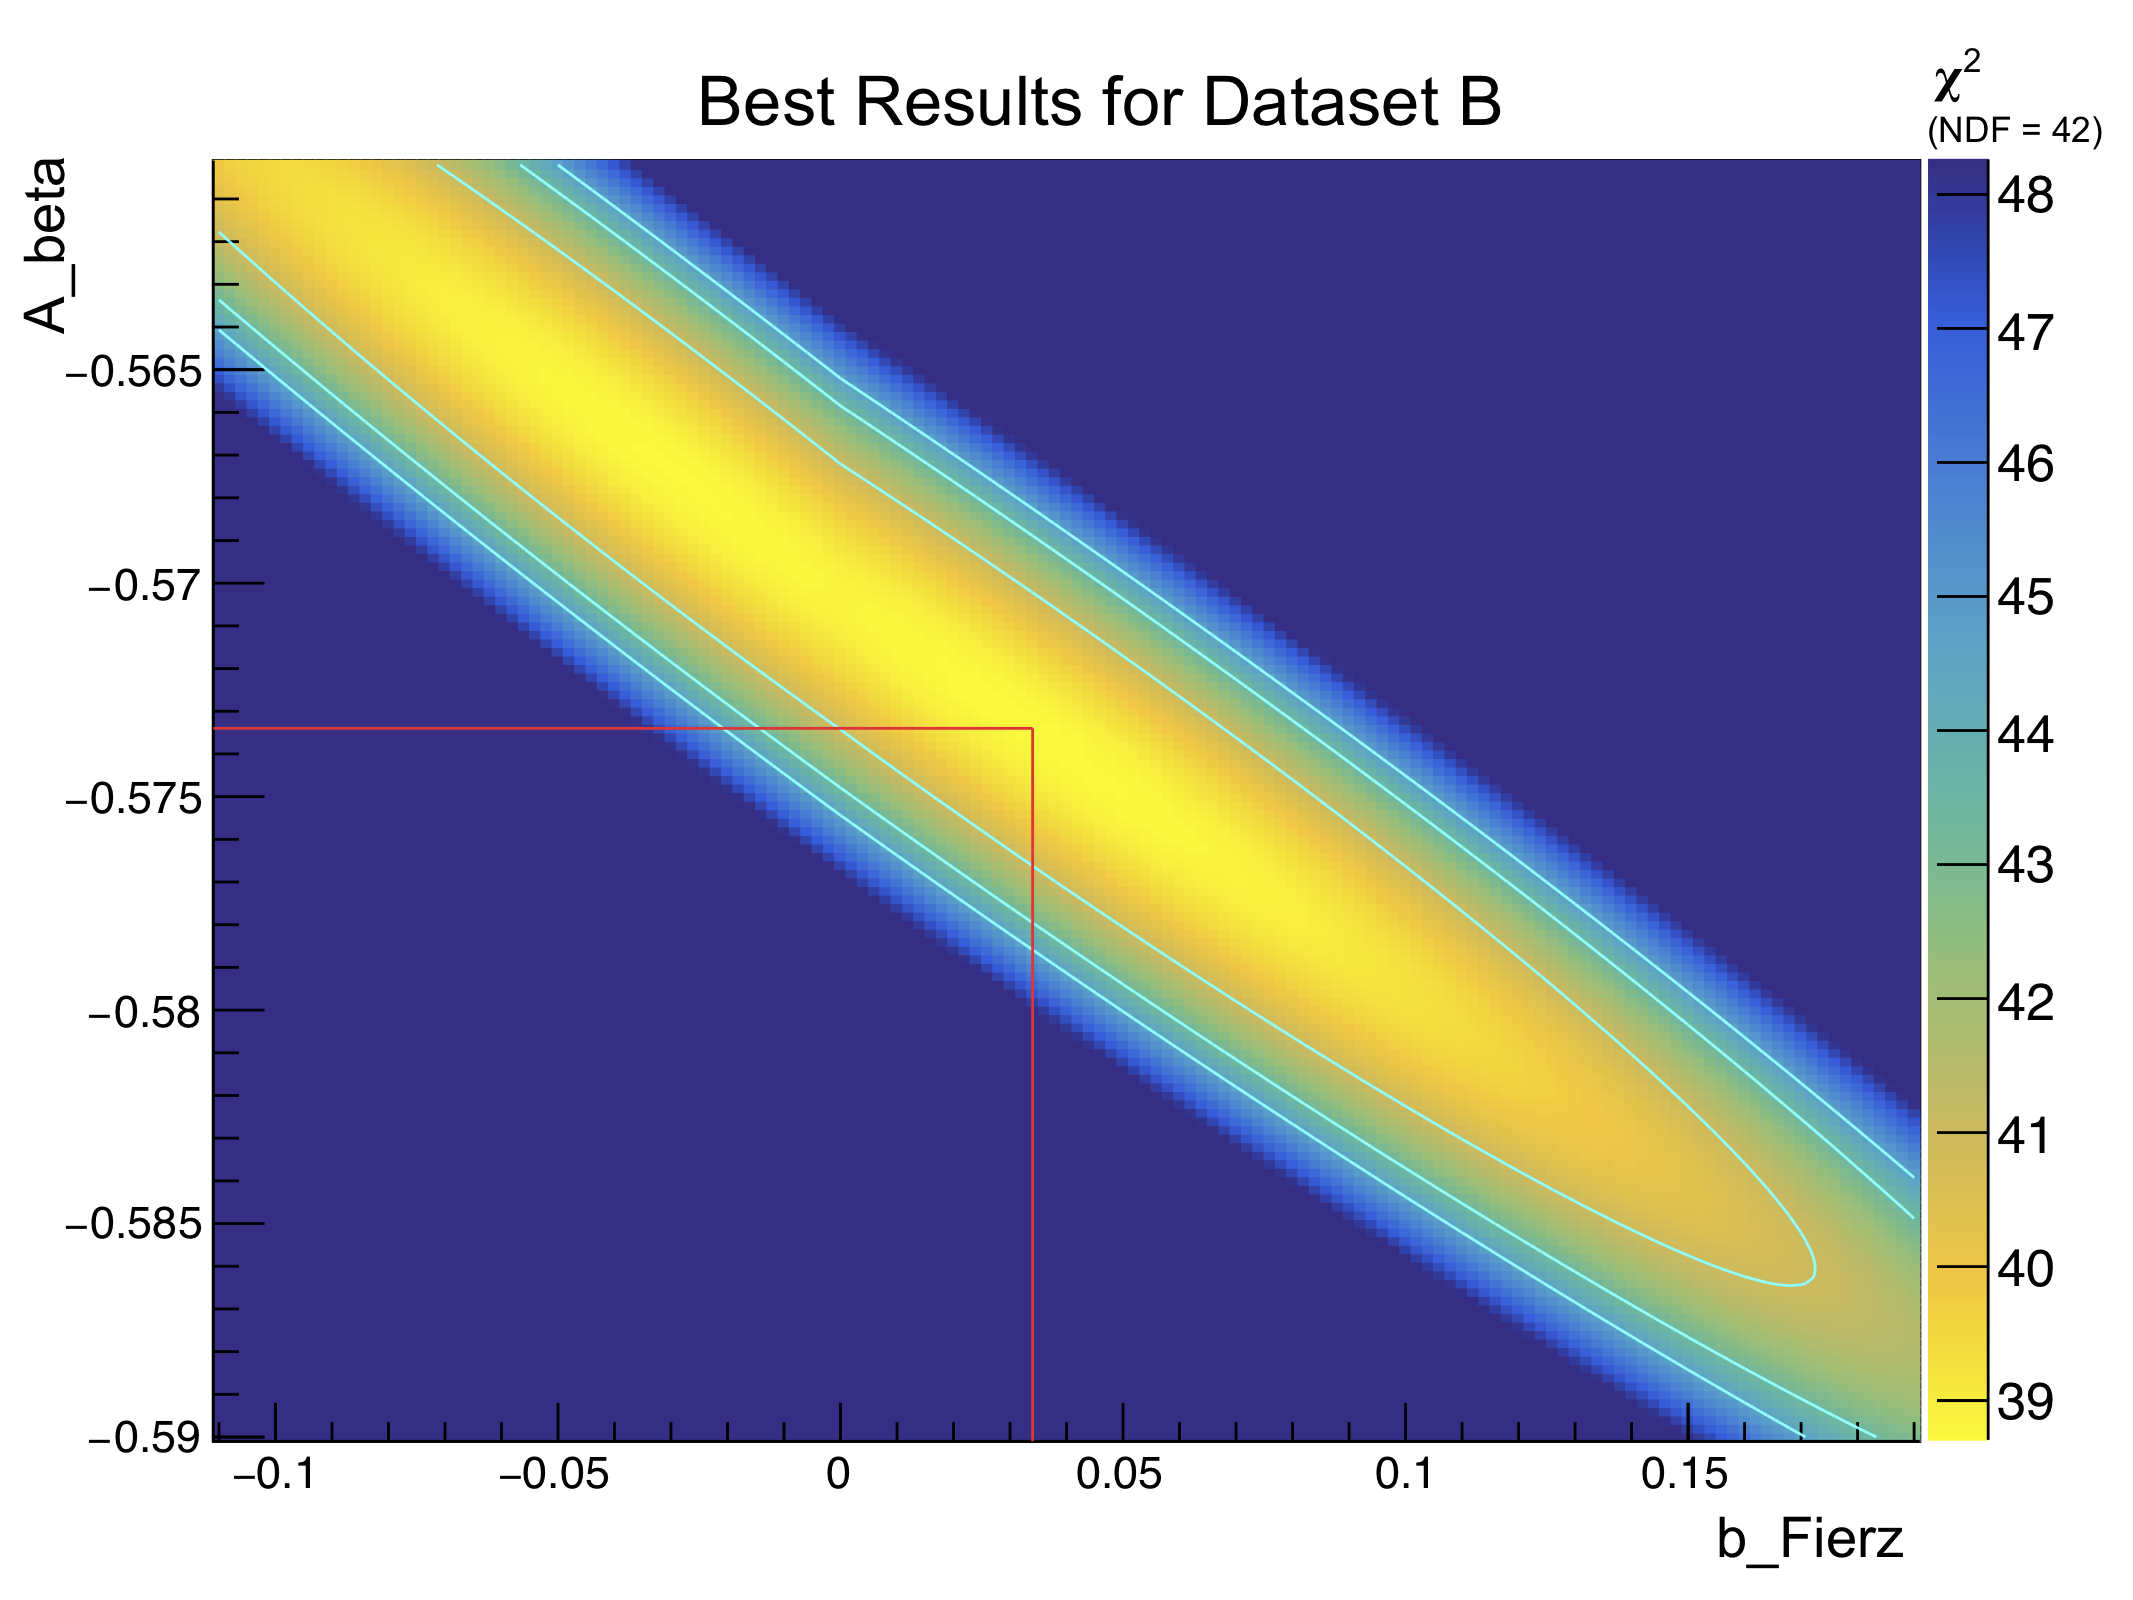
\includegraphics[width=.999\linewidth]
	{Figures/Chi2_2D_SetB.png}
	\note{Systematic uncertainties are evaluated by adjusting parameters and creating a new (set of) chi2 maps very much like this one.}
%	\note[color=tag]{On the per-dataset $\chi^2$ maps and SR asymmetries, go through and write descriptions for the goddamn pictures.}
	\caption[$\chi^2$ Map for Runset B]{A $\chi^2$ map to compare data from Runset B to a parameter space of $\Abeta$ and $\bFierz$ values.  The contours show 1$\sigma$, 90\%, and 95\% statistical confidence intervals.}	
	\label{fig:2dchi2_setB}
\end{figure}
%
\begin{figure}[h!tb]
	\centering
	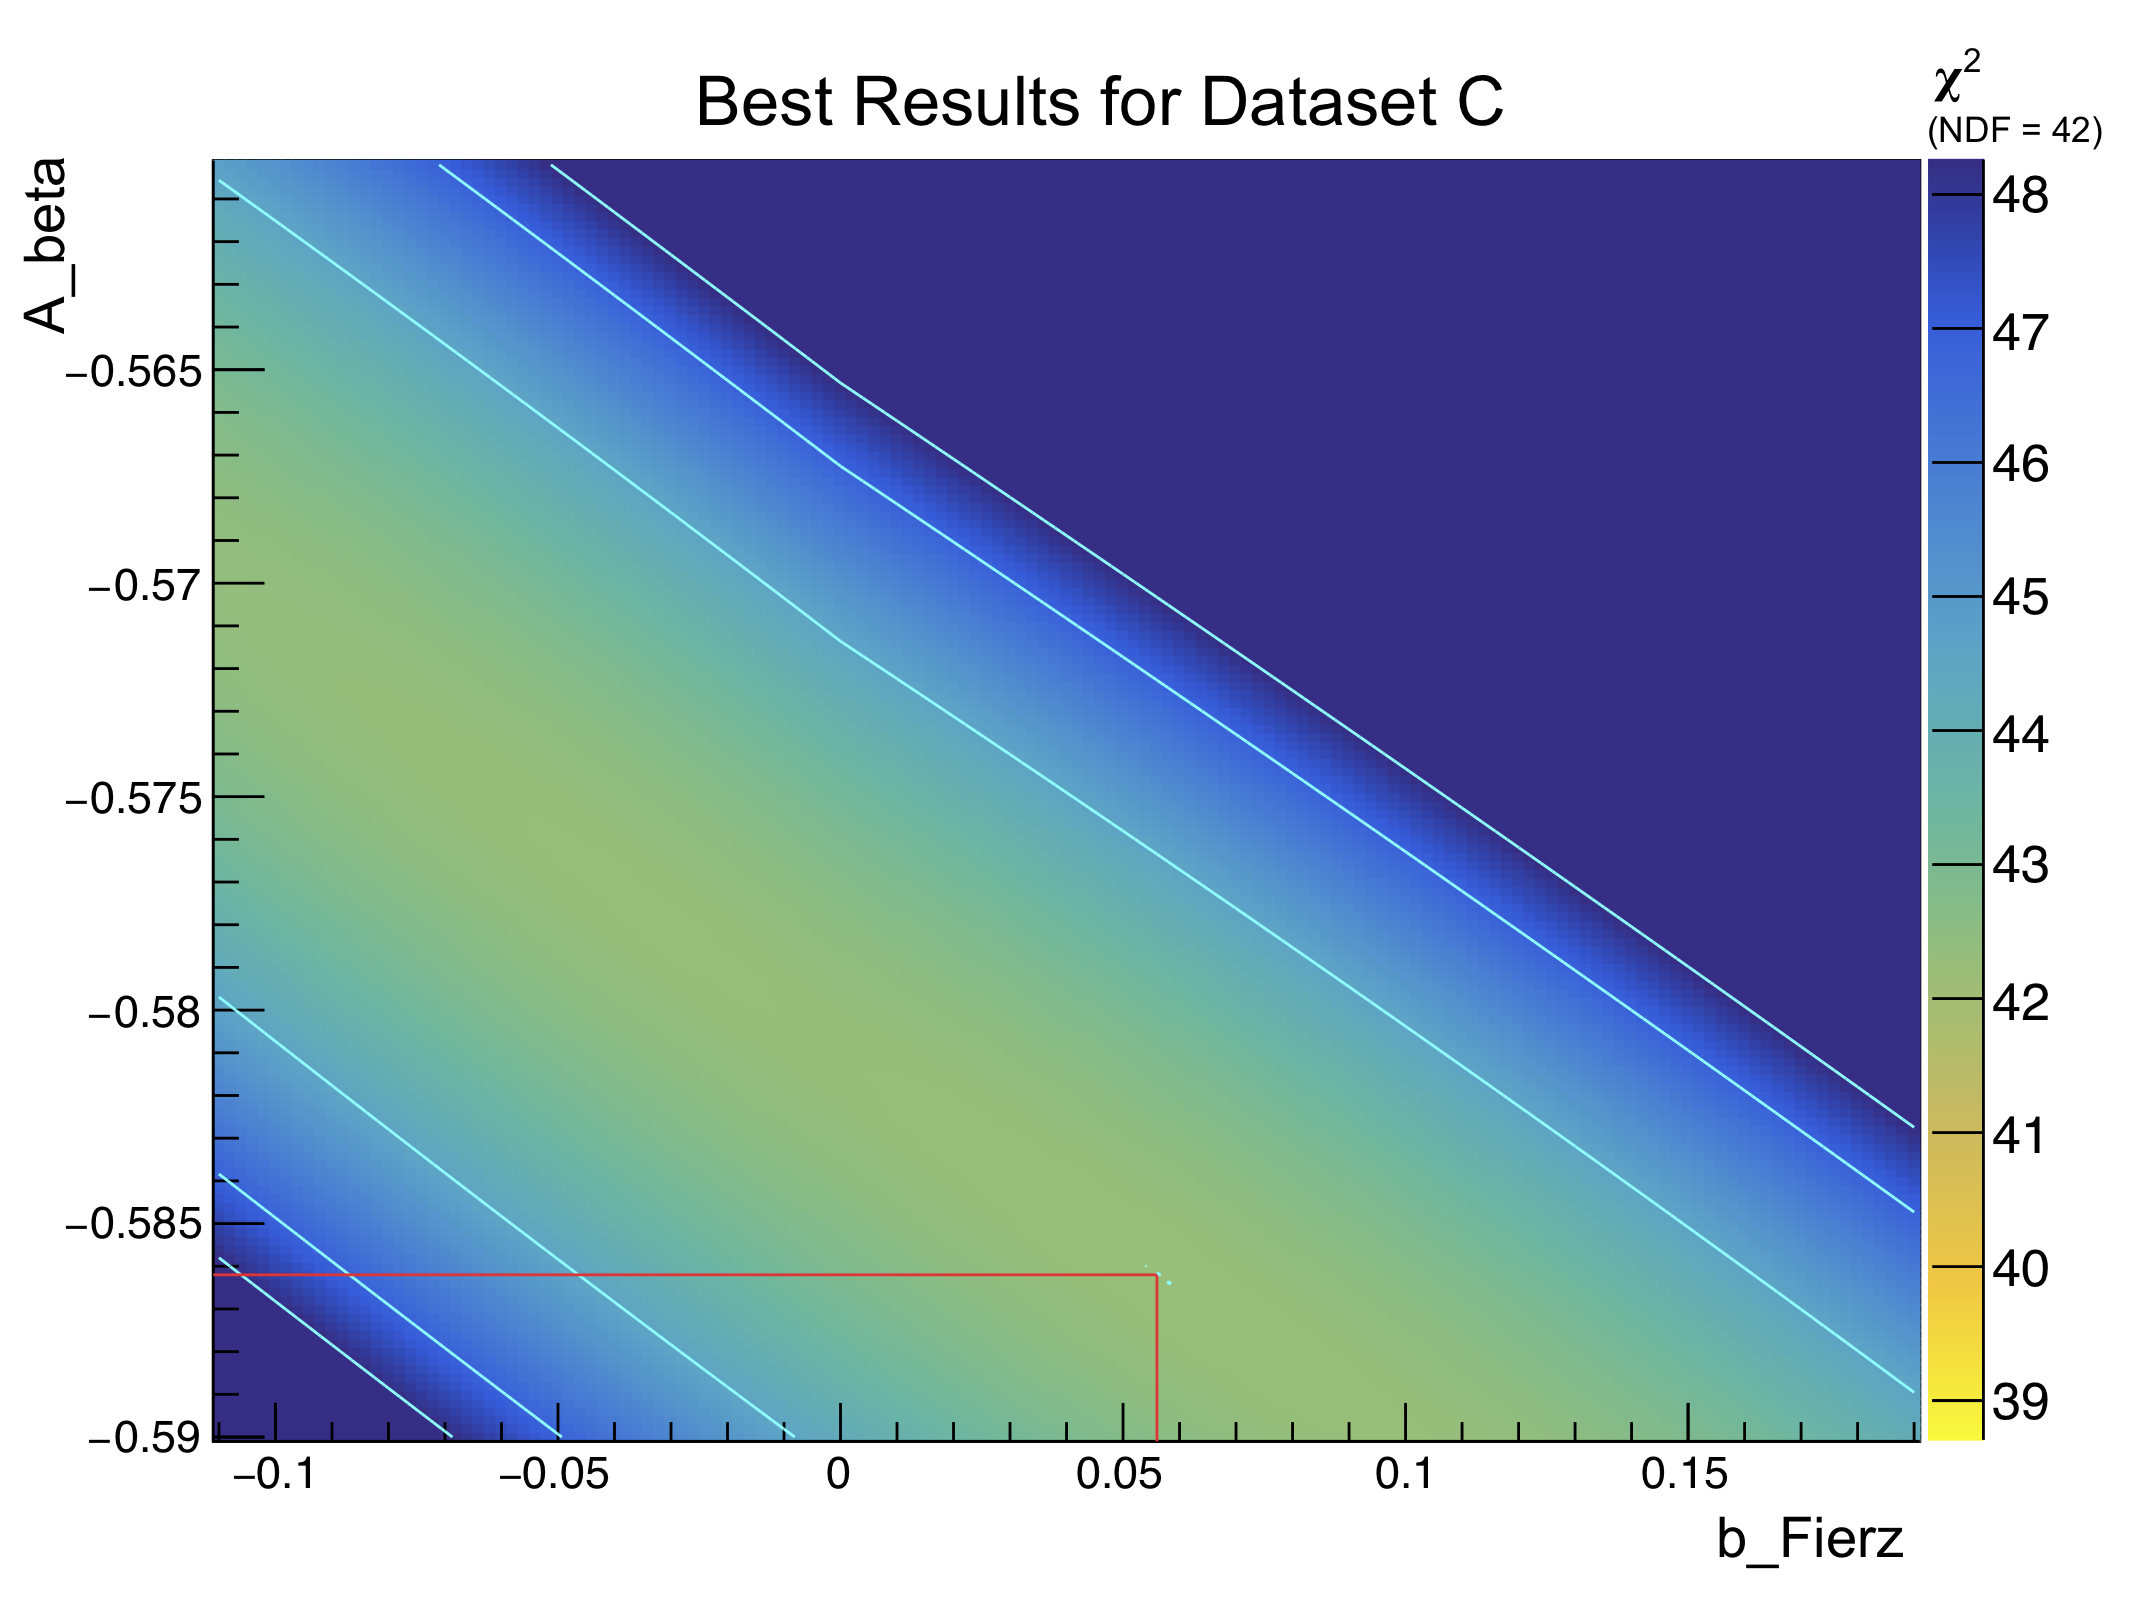
\includegraphics[width=.999\linewidth]
	{Figures/Chi2_2D_SetC.png}
	\caption[$\chi^2$ Map for Runset C]{A $\chi^2$ map to compare data from Runset C to a parameter space of $\Abeta$ and $\bFierz$ values.  The contours show 1$\sigma$, 90\%, and 95\% statistical confidence intervals.}	
	\label{fig:2dchi2_setC}
\end{figure}
%
\begin{figure}[h!tb]
	\centering
	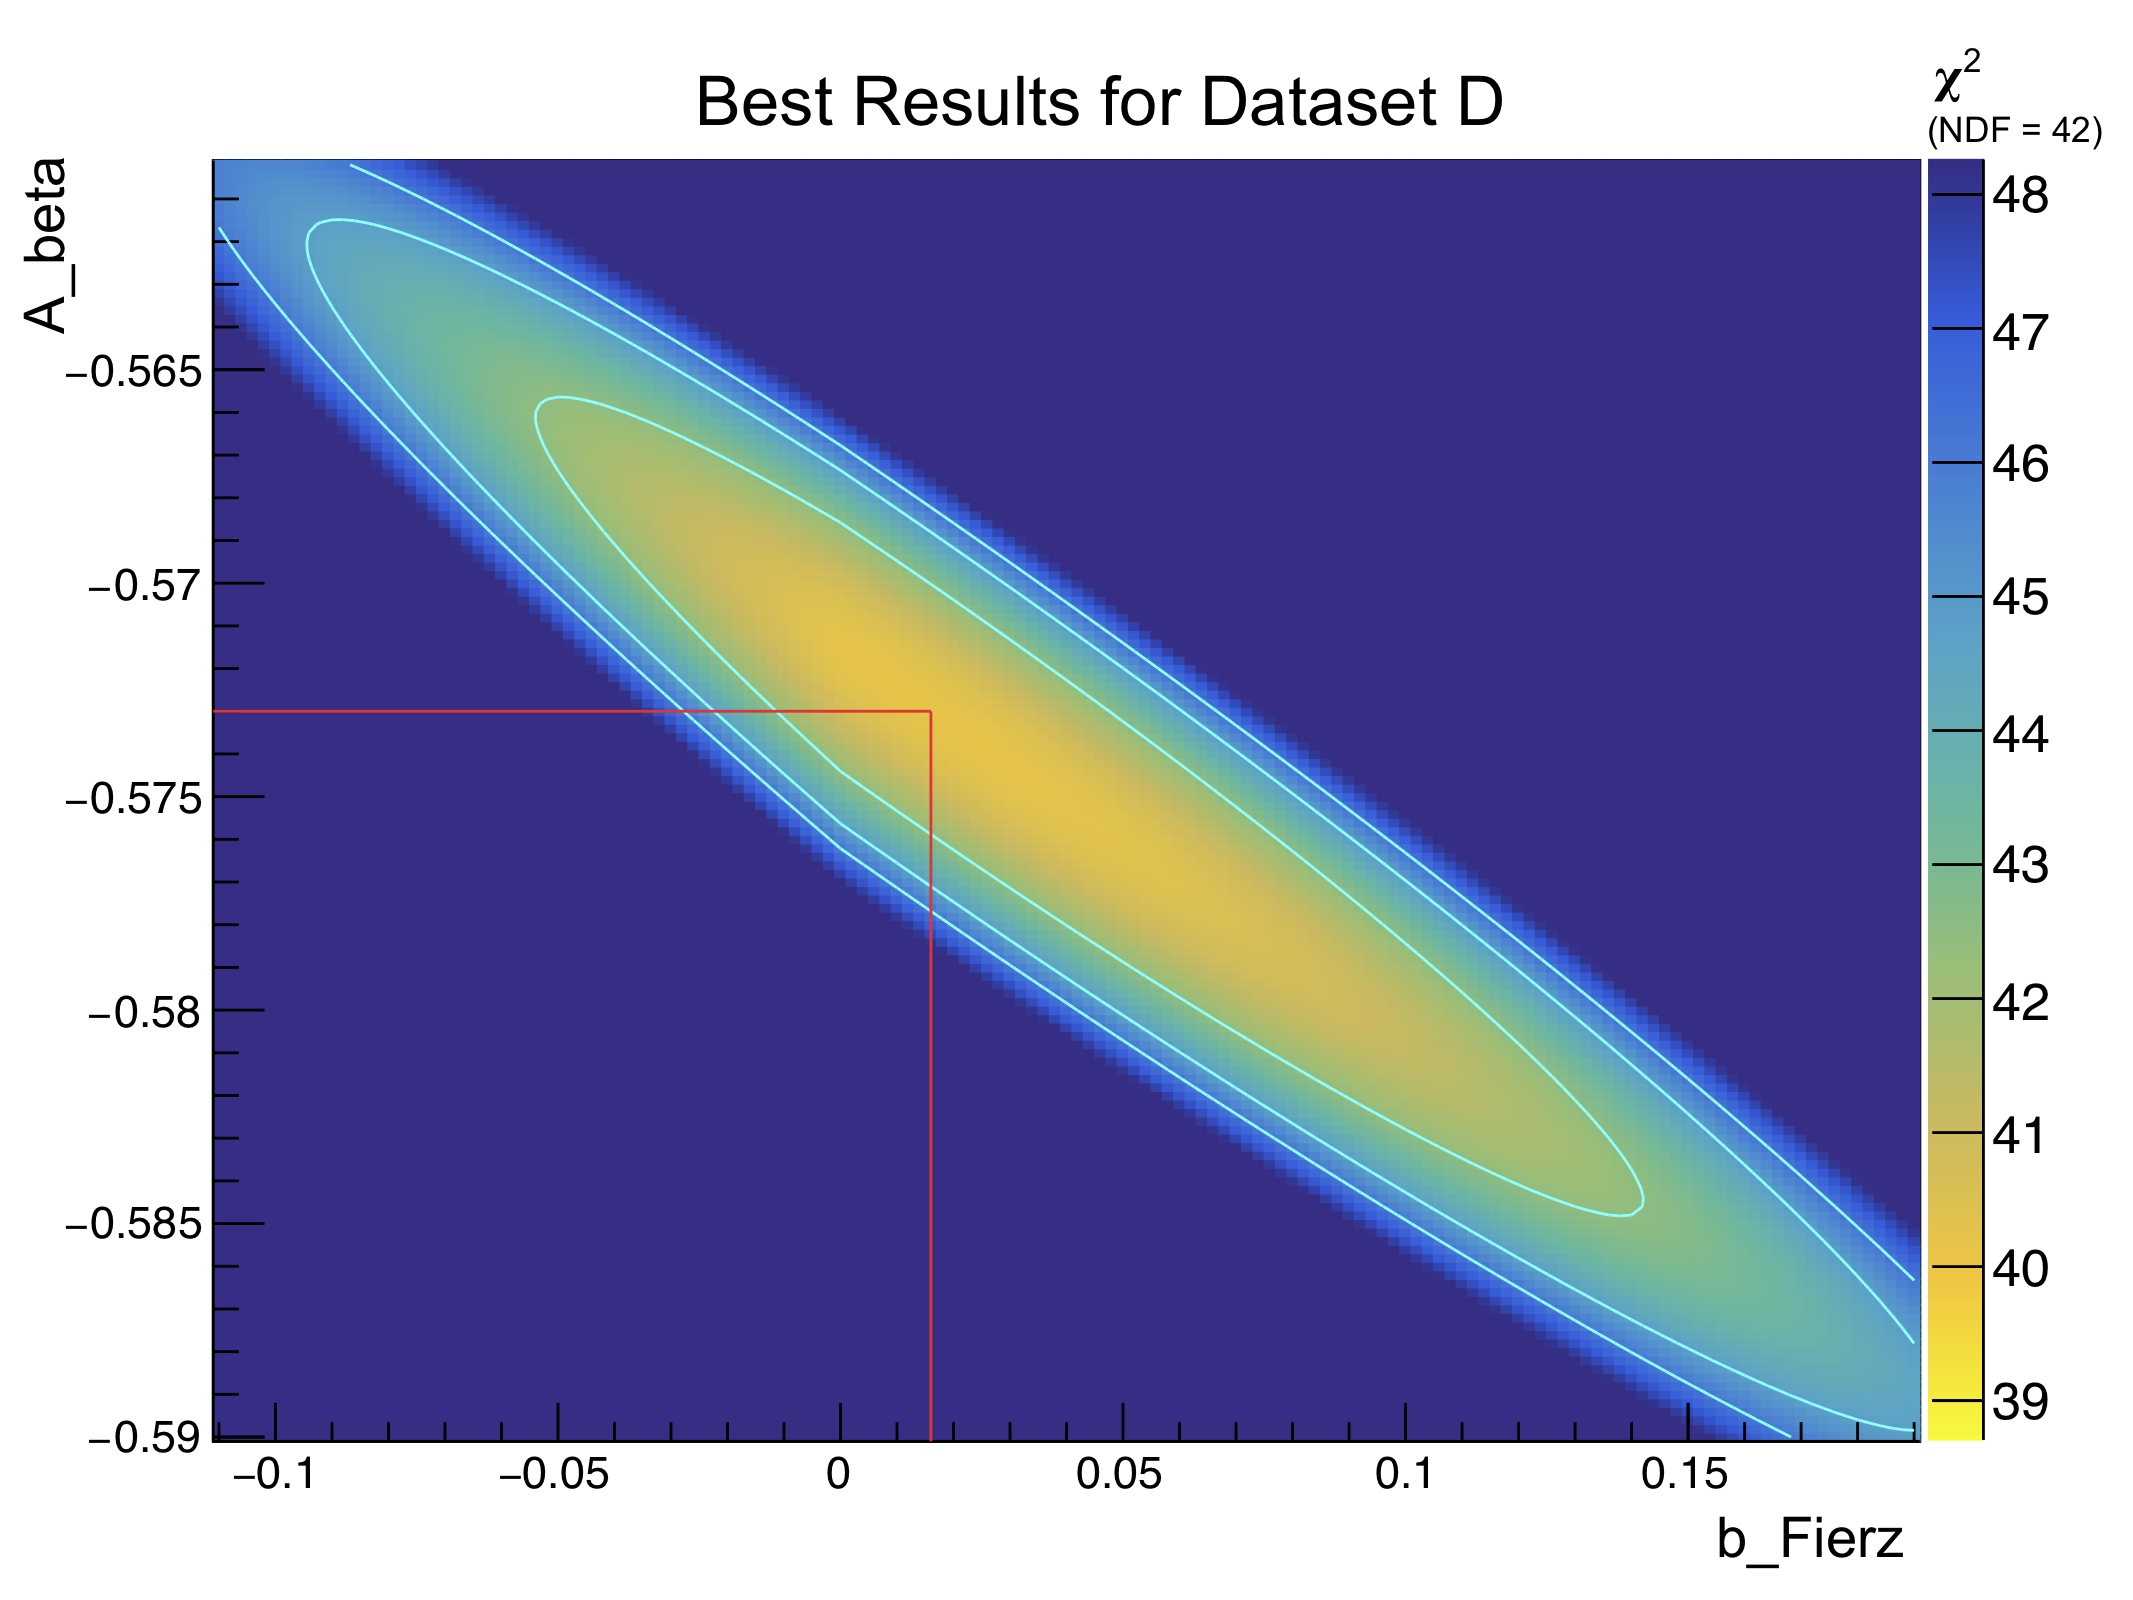
\includegraphics[width=.999\linewidth]
	{Figures/Chi2_2D_SetD.png}
	\caption[$\chi^2$ Map for Runset D]{A $\chi^2$ map to compare data from Runset D to a parameter space of $\Abeta$ and $\bFierz$ values.  The contours show 1$\sigma$, 90\%, and 95\% statistical confidence intervals.}	
	\label{fig:2dchi2_setD}
\end{figure}



\note{We can do this whole chi2 map thing again for real- and simulated data sets with different values of parameters that we vary as *systematics.*  Note how the best values of $\Abeta$ and $\bFierz$ change when each of the systematics are varied.}

%%%%That old list:
%%%%\begin{itemize}
%%%%	\item For each of those 3 simulations, sort the ``good'' data according to emission angle relative to the detector.  Do each detector individually.  For both polarizations.
%%%%	\item We can do this whole thing again for simulated data sets with different values of parameters that we vary as systematics.  Note how the best values of $\Abeta$ and $\bFierz$ change when each of the systematics are varied.
%%%%\end{itemize}
%%%%


\FloatBarrier
\section{Evaluation of Systematic Effects}
\label{section:systematics}
\subsection{Beta Scattering}
%\section{Quantifying the Effects of Backscatter with Geant4}
\label{section:scattering_systematics}
%\note[color=org]{This content got moved over *there*.  (ie, Section~\ref{sec:bs}.)}
The methodology used to simulate and model scattered events is described in Section~\ref{sec:bs}.  To evaluate the systematic effect on the final measurements arising from incomplete knowledge of how much beta scattering is present (i.e., how well we can trust the simulation to correctly model the amount of scattering), 
%To evaluate the systematic effects arising from incomplete knowledge of how much beta scattering is present, 
two sets of $\chi^2$ maps very much like those in Section~\ref{sec:comparing_data_sims} are created, with the amount of scattering varied by one standard deviation.  This does not require a new simulation;  instead, for the three high statistics G4 simulations varying the BSM scalar coupling, all events passing the cuts are categorized into `unscattered and forward-scattered' events, `sidescattered' events, and `backscattered' events, depending on a comparison of the beta's emission angle to the detector in which it was eventually observed, as shown in Fig.~\ref{fig:soe_tof_vs_costheta}.

The contribution from unscattered and forward scattered events is not allowed to vary, but the weights attributed to sidescattered and backscattered events was varied by $\pm 10\%$ and $\pm 5.1\%$ (respectively) relative to their `best' values.  Fig.~\ref{fig:asymmetry_scattering} clearly shows the change in superratio asymmetry produced by this variation in the amount of scattering.  The method by which it was determined how much the scattering weights should be allowed to vary is described in the supplementary material of a recent publication by the collaboration~\cite{ben_Abeta}.
\begin{figure}[h!tb]
	\centering
	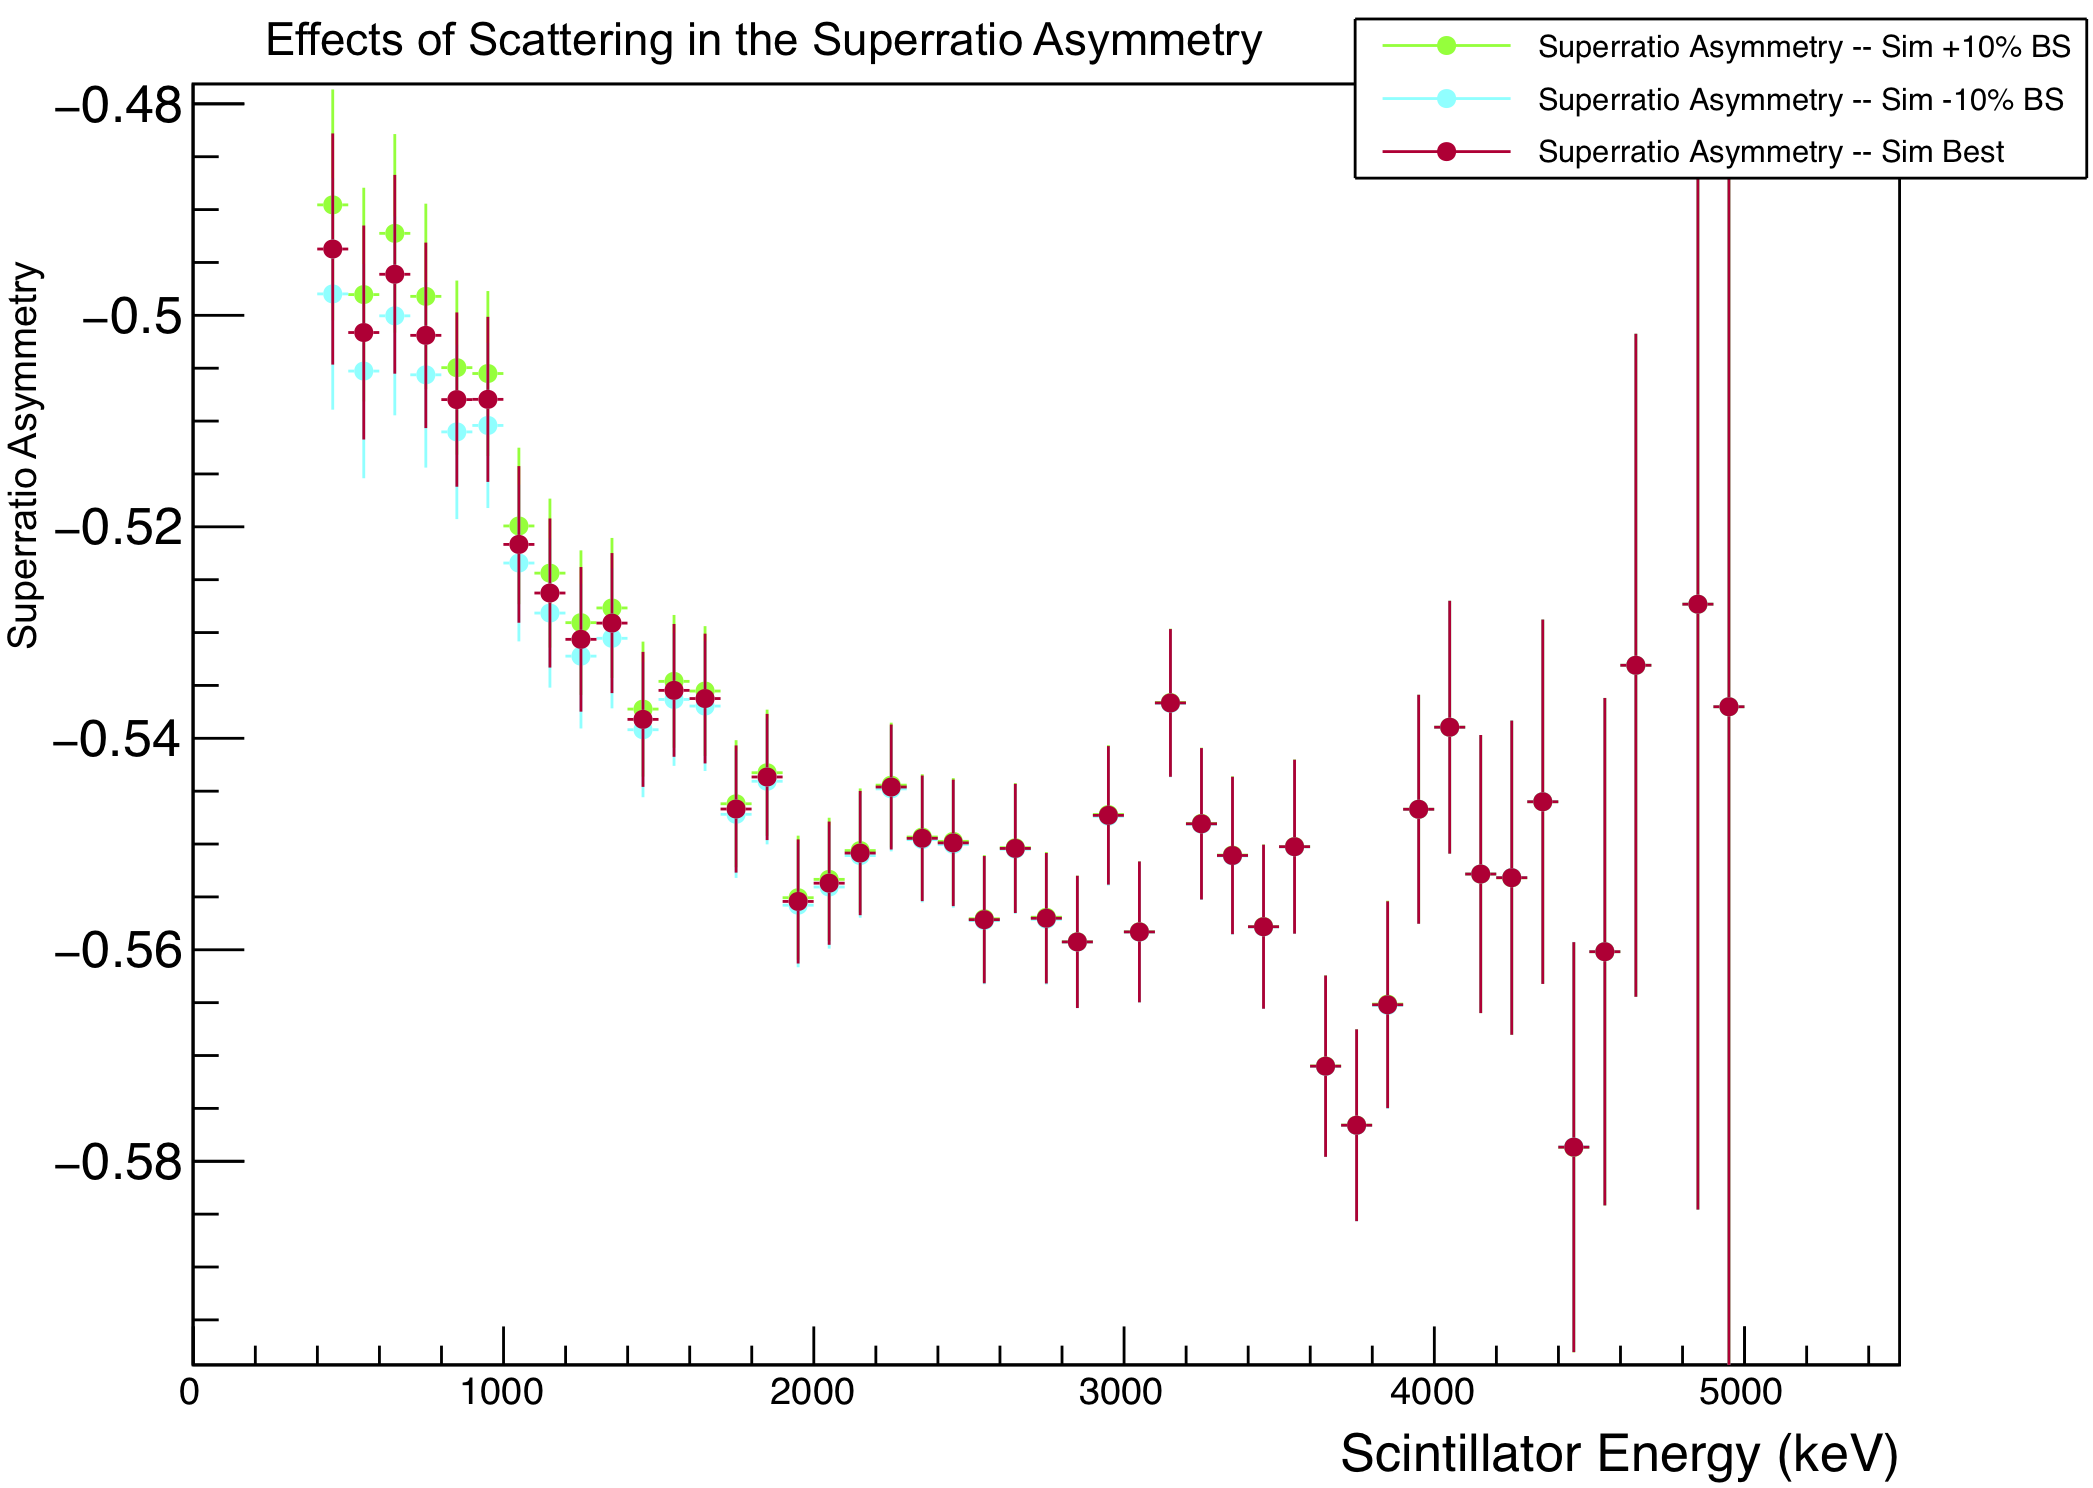
\includegraphics[width=.999\linewidth]
	{Figures/ScatteringEstimate.png}
%	\note{I got it out of the Sim\_to\_Asym directory, so that's where I have to go looking to see how I made it and/or make a new one. .... nope, the new one is from Fit_2D.}
%%%%%	\note[color=jb]{John on Section~\ref{section:scattering_systematics} ``Quantifying the Effects of Backscatter with Geant4'':
%%%%%\\...\\
%%%%%Fig.~\ref{fig:asymmetry_scattering} illustrates the distortions in the energy dependence of Abeta
%%%%%that mimics effects of bFierz. A generic 10\% uncertainty assigned to
%%%%%the GEANT4 similation of backscatter produces the largest systematic
%%%%%uncertainty in bFierz. Based on this result, the collaboration is
%%%%%attempting to improve the
%%%%%experimental design to use lower-Z materials to improve this systematic.
%%%%%\\
%%%%%(I.e. that's all you need to say. The figure tells the story.)}
%
	\caption[Scattering Effects in the Asymmetry]{The amount of scattering is adjusted by one standard deviation in both directions, and the results to the superratio asymmetry are plotted.  The bulk of the effect occurs at lower energies, where sensitivity to $\bFierz$ is at its highest.}	
	\label{fig:asymmetry_scattering}
\end{figure}
%%%\note{Oh fuck.  Oh fuck oh fuck oh fuck.  $5.1\%$ is actually a $2\sigma$ limit.  I guess $10\%$ is still basically just a guess though.  Still, this kills like half of the systematic error.  I'll have to re-evaluate this later.}
Since errors in evaluating both side-scatter and backscatter arise from limitations on how well Geant4 is expected to perform, it is not clear how correlated these errors are, but it seems foolish to suppose they should not be correlated at all.  Therefore, the conservative assumption that the two are \emph{fully} correlated is taken, and the errors from side-scatter and backscatter are added \emph{linearly} to one another before being combined in quadrature with the other uncertainties.  

As this is the dominant systematic error, the TRINAT collaboration is working to improve the experimental design to use lower-Z materials to reduce the size of this effect.




\subsection{Detector Calibrations and Thresholds}
\subsubsection{Scintillators}
\note{I could and probably *should* add a description of the scintillator threshold uncertainty evaluation.  But I'm going to skip that for Round 1 and see if anybody notices.}
The two plastic scintillators were calibrated by the collaboration using online data, with reference points from the beta spectrum endpoint and the compton edge arising from annihilation radiation.  Calibration was performed using only \emph{polarized} data, because the final measurements use only polarized data, and the scintillator gain is more stable in the absence of the stronger oscillating magnetic fields from the AC-MOT.  

A linear calibration is used, with
\bea
E_{\textrm{scint}} &=& \frac{1}{m}(Q_{\textrm{QDC}} - b), 
\eea
and the detector resolution arising from photon counting statistics is given by
\bea
\sigma &=& \sqrt{\lambda E_{\textrm{scint}}}.
\eea

During online data collection, one QDC module failed abruptly and had to be replaced.  As a result, the collected data is calibrated separately before and after the module failure, and the calibrations change slightly at this time. The methodology used is described in detail within~\cite{ben_thesis}, so the results will simply be stated here in Table~\ref{table:scintcal}.
% !TEX root = ../thesis_main.tex
%
%
%
\begin{table}[h!!!!t]
	\begin{center}
	\begin{tabular}{| l l || l | lcl | lcl | lcl |}
			\multicolumn{2}{l}{ Runsets  }{ } & \multicolumn{1}{  c  }{ } & 
				\multicolumn{3}{  c  }{ b } &  \multicolumn{3}{   c  }{ m } &  \multicolumn{3}{   c  }{ $\lambda$ }  \\
			\cline{1-12}
			\multirow{2}{*}{EA, EB} & \multirow{2}{*}{RA, RB}   
								&  Top    & \,\,110.0 & \!\!$\!\! \pm  \!\!$\!\! & 0.3   & \,\,0.3985  & \!\!$\!\! \pm  \!\!$\!\! & 0.0004 & 1.55 & \!\!$\!\! \pm  \!\!$\!\! & 0.09  \\
								&& Bottom & \,\,142.0 & \!\!$\!\! \pm  \!\!$\!\! & 0.3   & \,\,0.4234  & \!\!$\!\! \pm  \!\!$\!\! & 0.0004 & 1.28 & \!\!$\!\! \pm  \!\!$\!\! & 0.08  \\
			\cline{1-12}
			\multirow{2}{*}{EC, ED} & \multirow{2}{*}{RC, RD, RE} 
								&  Top    & \,\,110.7 & \!\!$\!\! \pm  \!\!$\!\! & 0.2  & \,\,0.3883  & \!\!$\!\! \pm  \!\!$\!\! & 0.0004 & 1.42 & \!\!$\!\! \pm  \!\!$\!\! & 0.08 \\
								&& Bottom & \,\,143.0 & \!\!$\!\! \pm  \!\!$\!\! & 0.3  & \,\,0.4132  & \!\!$\!\! \pm  \!\!$\!\! & 0.0004 & 1.32 & \!\!$\!\! \pm  \!\!$\!\! & 0.08 \\
			\cline{1-12}
	\end{tabular}
	\end{center}
	\note{Maybe this thing needs units?}
	\caption[Scintillator Calibrations]{Scintillator Calibrations}
	\label{table:scintcal}
\end{table}



To evaluate the systematic effects associated with the scintillators' calibrations, the calibration for each scintillator is adjusted independently to produce energy measurements that are higher by one standard deviation, and lower by one standard deviation, and the resulting changes to the $\chi^2$ map's $\Abeta$ and $\bFierz$ centroids is measured.  For this, the datasets corresponding to both sets of calibration numbers have their calibrations adjusted simultaneously, but each individual scintillator is treated separately.  There is no reason to think the two scintillators' calibration accuracies should be correlated, so errors resulting from a changed scintillator calibration are added to one another in quadrature.

%%%%Uncertainties resulting from an inaccurate scintillator calibration are added in quadrature for the final result, because there is no reason to think the two scintillators' calibration inaccuracies should be correlated.
%%%%
%%%%Because it is not immediately intuitively obvious how different a calibration mistake on both scintillators might change the resulting measurement of $\bFierz$, 
%%%%There is no reason to believe the errors in calibration should be correlated, so 

\subsubsection{DSSD Radius, Energy Threshold, Agreement}
%\section{BB1 Radius, Energy Threshold, Agreement}
\label{section:bb1_systematics}
%\note[color=tag]{Write section dssd systematics evaluation.}
Several parameters relating to our choice of cuts relating to DSSD calibrations are varied within both the experimental data and the simulated data to which it is compared.  The detection radius, the overall energy threshold, the strip-by-strip SNR, and the energy and timing agreement (See Ch.~\ref{sec:dssd_cuts}) are each adjusted separately at the start of data processing, and the changes are propagated through to a final $\chi^2$ map.  

The changes to measured values of $\bFierz$ and $\Abeta$ from these adjustments are comparatively small, and the errors are believed to be uncorrelated, so they are added in quadrature to the total systematic uncertainty.

%Although they don't all have an intuitively clear name, 

%%
%%BB1 radius cut can help to eliminate scattered events.  Energy threshold selection and statistical agreement between BB1 detectors' energies only makes a small effect on results.  BB1 radius itself has a pretty big effect on the result, but we can at least just G4 it away.  The remaining systematic effect is pretty small.  
\note[color=jb]{JB:  I hope the discussion is clear in your head.  Any effect that relies on scattering computation in G4 should have an uncertainty on order 10\% of the correction -- hopefully you are keeping a distinction here between the finite geometry acceptance (which I guess is exact) scattering off the collimator.}
\note[color=jb]{As per JB's comment in section~\ref{thesisconventionjb}:   ``statistical agreement between BB1 X and Y detectors' energies only makes a small effect on results" does not need the technical details beyond that statement."}
	
\missingfigure{Surely this requires at *least* one image of the pixelated BB1 data.  Maybe some of a few waveforms and energy distributions too.  ....Feels like cheating to include some of that stuff, since Ben was the one who actually used it mostly.}
\note[color=jb]{JB on missing figure:  ``if you used such an image as part of your uncertainty estimate, yes [include it]''}

\note{Remember:  There's noise applied to simulated BB1s, matching some spectrum.}
\note{This probably should go somewhere else:  "In the end, we get our results from the scintillator energy only, without summing the BB1 energy back in.  Energy absorbed in DSSDs is only used as (a) a tag for events, and (b) contributing to the total beta energy loss before the beta arrives at the scintillator."}
\note[color=jb]{JB:  The simulations of course include it event-by-event, not just a minimally ionizing average loss.}

%%%% --- * --- %%%%
\subsection{The Atomic Cloud}
%\section{Lineshape Reconstruction}
\label{sec:lineshape_results}
%\note[color=tag]{(Re-)Write sections systematics from the cloud.}
\note[color=org]{A lot of this content has gone into (Section~\ref{sec:responsefunction}) instead.  I really need to just mention it here (Sec.~\ref{sec:lineshape_results}) and give an indication of how good the result is.  Then evaluate stuff.}
Uncertainties relating to the position, size, motion, and expansion of the atomic cloud are evaluated using the response function, which is implemented as described in Ch.~\ref{sec:responsefunction}. To evaluate how well the simple monte carlo + response function (SMC+RF) performs in evaluating uncertainties, the relationship between how the SMC+RF and the full G4 simulation changes when a BSM parameter is adjusted is considered in Fig.~\ref{fig:lineshape_demo}.

\begin{figure}[h!!!t]
	\centering
	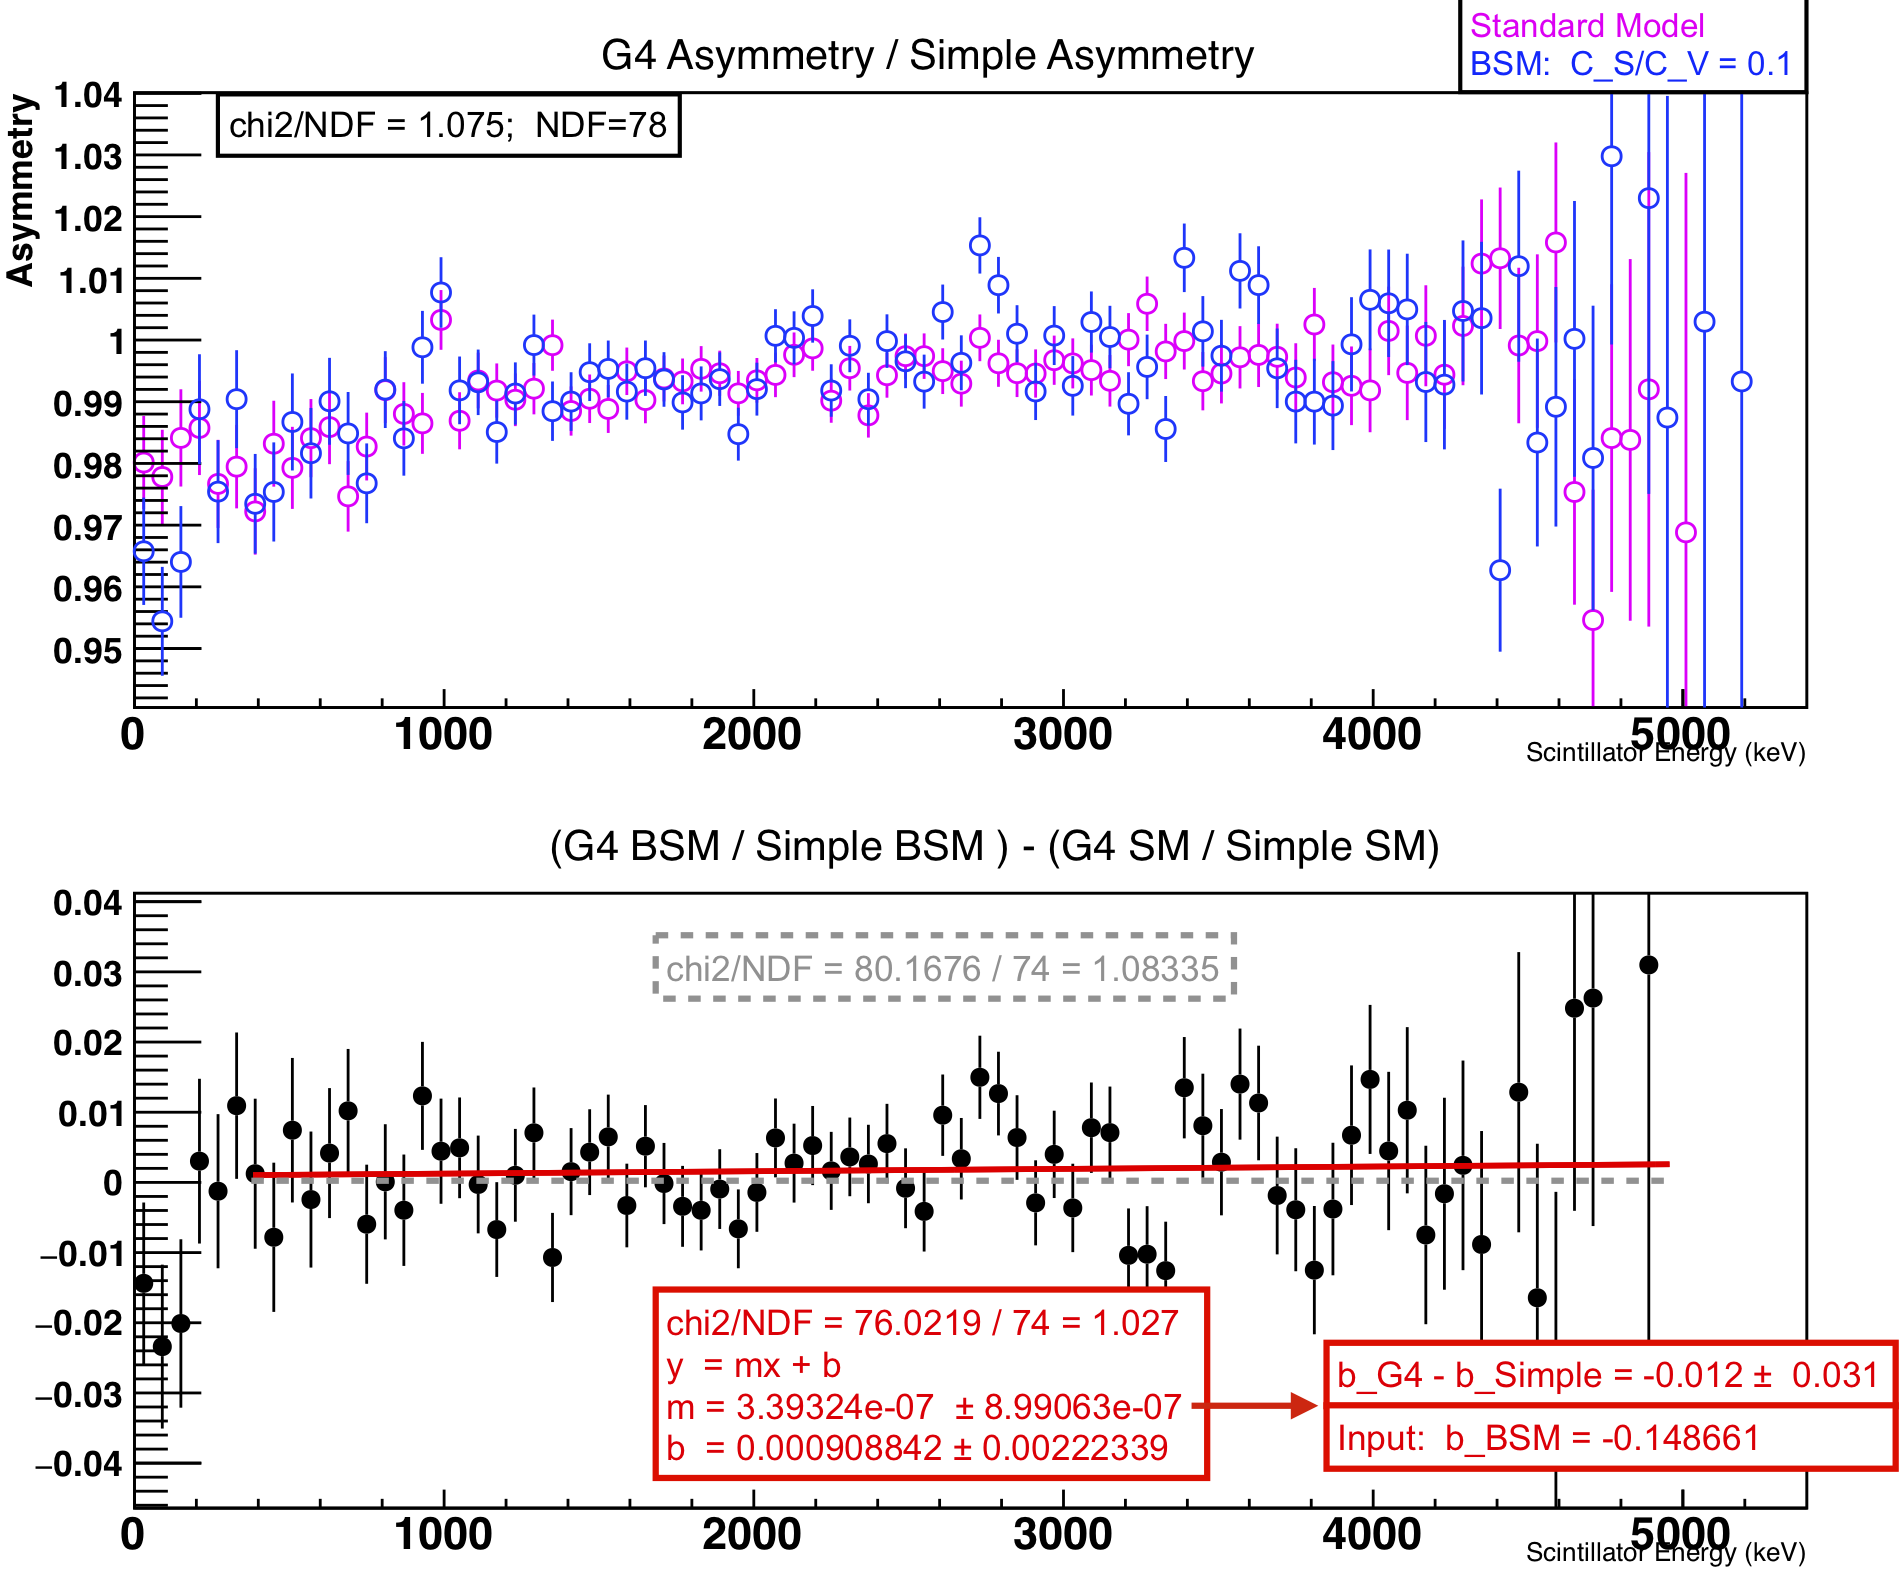
\includegraphics[width=.999\linewidth]
	{Figures/LineshapeDemo_quasiprelim.png}
\note{This is a horrible and ugly picture, and it should be replaced.}
\caption[Response Function Comparison]{Superratio asymmetries generated by G4 and SMC+RF are compared against one another for a change in BSM parameters.  The results show a consistent behaviour when the value of $\bFierz$ is adjusted, suggesting that the SMC+RF can safely be used to evaluate systematic effects such as those arising from a change in cloud position.
%I'm not actually sure if this picture shows what I want it to.  The point is, if I apply this rough lineshape to stuff that I SimpleMC-ed, then I can evaluate that way various systematic effects that would be time-consuming to actually simulate with G4.  This picture is  *supposed* to be a demonstration that this approach actually works... 
}    	
	\label{fig:lineshape_demo}
\end{figure}

To evaluate the propagated systematic effects arising from our knowledge of the cloud position, the simple monte carlo is used to generate events originating at points chosen randomly from the distributions produced by linear interpolation of the parameters in Table~\ref{table:cloudpositions}, with each parameter describing the distribution allowed to vary in accordance with its stated uncertainty, assuming gaussian-distributed errors.  The results for each of the three datasets are shown in Fig.~\ref{fig:Abeta_position_err} for $\Abeta$ and Fig.~\ref{fig:bFierz_position_err} for $\bFierz$.


\begin{figure}[h!!tb]
	\centering
	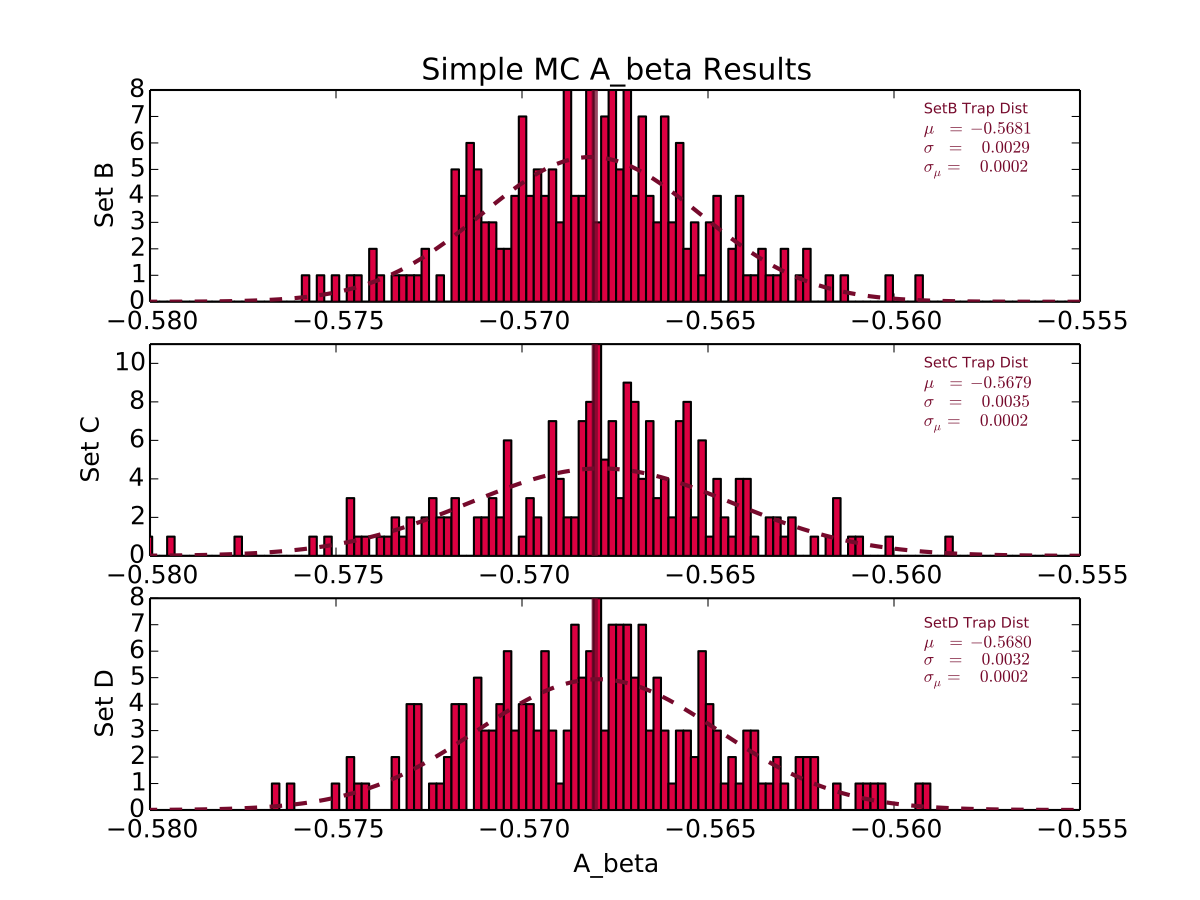
\includegraphics[width=.999\linewidth]
	{Figures/Position_Err_Abeta.png}
	\caption[$\Abeta$ Position Error]{Estimated offset and uncertainty in $\Abeta$ resulting from an imperfectly centred cloud of finite size, and the uncertainty and variation within these parameters.  Evaluated by using the SMC+RF method.}	
	\label{fig:Abeta_position_err}
\end{figure}

\begin{figure}[h!!tb]
	\centering
	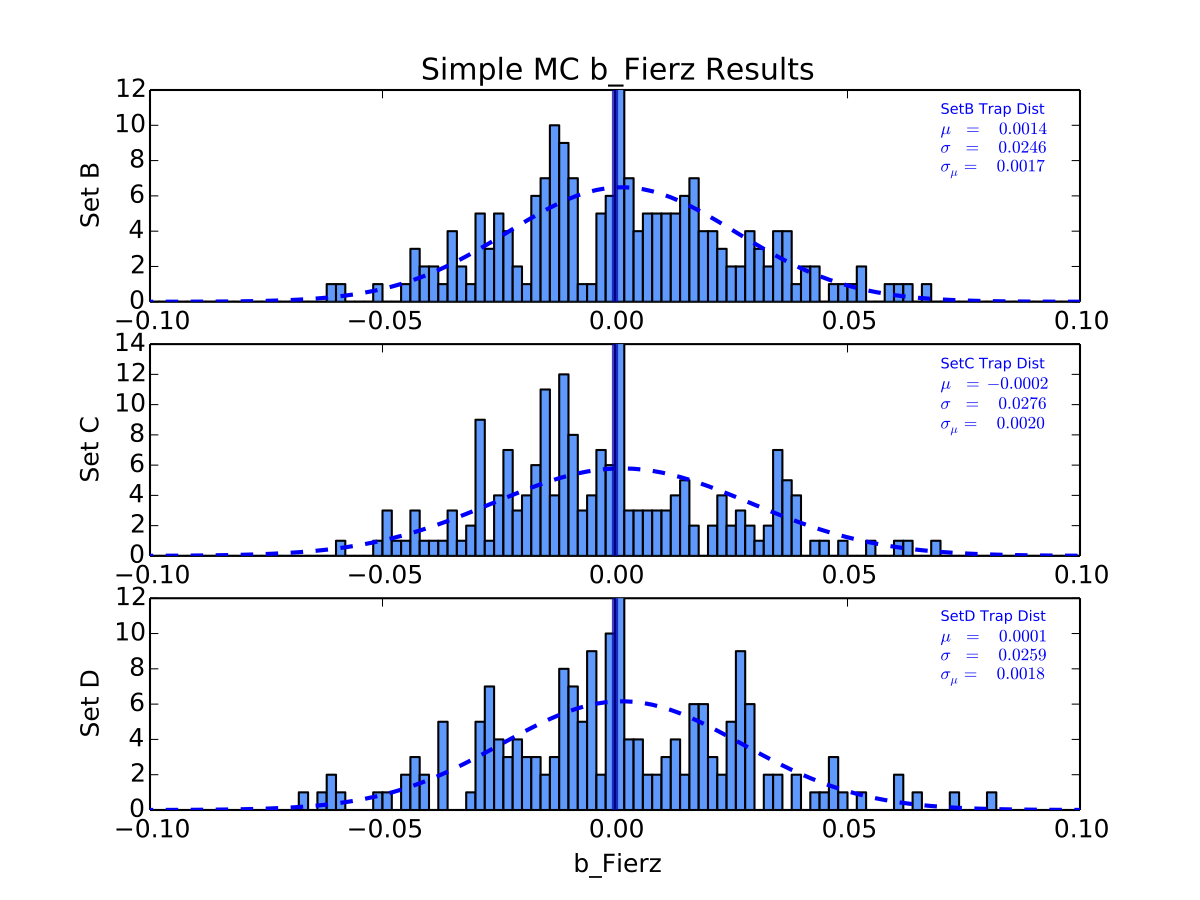
\includegraphics[width=.999\linewidth]
	{Figures/Position_Err_bFierz.png}
	\caption[$\bFierz$ Position Error]{Estimated offset and uncertainty in $\bFierz$ resulting from an imperfectly centred cloud of finite size, and the uncertainty and variation within these parameters.  Evaluated by using the SMC+RF method.}		
	\label{fig:bFierz_position_err}
\end{figure}


%%%\note[color=jb]{John on Ch.~\ref{sec:lineshape_results} ``Lineshape Reconstruction'':
%%%%\\...\\
%%%%I can only recommend now including what you've written (your extensive work on the rest you
%%%%documented well in your TRINAT meeting reports have):
%%%\\...\\
%%%Keep the details you have in 5.6 and Fig. 5.2. Fix Fig. 5.2 caption.
%%%\\...\\
%%%Keep 5.6.2 as the conclusion of 5.6.1, omitting the final sentence
%%%on bremsstrahlung which is evaluated analytically now in 5.6.3.
%%%State clearly something like
%%%"The goal of the simple MC was fine-- a method to evaluate uncertainties
%%%without extensive simulation.
%%%However, difficulties including parameterizing the lineshape made its implementation less general, and
%%%extensive running of the full GEANT4 simulation for many small variations
%%%proved necessary."
%%%}	
%%%	
%%%Clifford tells us what to do.~\cite{clifford}.
%%%	
%%%\subsubsection{The Response Function -- What It Is and How It Works}
%%%Mono-energetic beta decay events are generated in GEANT4, which outputs an energy spectrum for unscattered and forward-scattered beta events in the detector.  These spectra are fit to a function to model the scintillator resolution, as well as energy loss in materials that the beta passed through before arriving at the scintillator.  These spectrum fits are performed for a set of beta energies, and parameters are extrapolated to be applied to betas emitted at intermediate energies.  Thus, the whole spectrum can be modeled.  Pictures will make this clearer. 
%%%	
%%%	
%%%
%%%%	\subsection{The Math-Specifics}
%%%%	I'll write down the specific functions I'm using, and the parameter values I'm using.  (Maybe this should go in an appendix instead?)  I'll describe the adjustments I make to the spectrum so that it can work even for the dataset where the scintillators' resolutions have changed.
%%%	
%%%\subsubsection{Cloud Parameter Uncertainty Evaluations with the Response Function}
%%%As it turns out, only cloud parameters were evaluated this way. \aside[color=jb]{JB:  so it's still critical to write down more of the lineshape work.}
%%%Trap position, size, sail velocity, temperature.  But then we varied the lineshape anyhow, to account for G4 doing a bad job of modelling the bremsstrahlung (sp?).
%%%%Thicknesses of the SiC mirror, the Be foil, and the DSSD.  Scintillator calibration.  
%%%\note[color=jb]{JB:  yes, brems strahlung is 'braking radiation' so gets 2 ss's. 
%%%the lineshape tail in any scintillator also includes backscattered events -- we are not claiming the 2-pixel cut is complete}
%%%	
%%%



%%%% --- * --- %%%%
\FloatBarrier
\subsection{The Response Function's Low Energy Tail}
%\note[color=tag]{Un-pinken/re-write section on the low energy lineshape tail.}
%\subsubsection{The low-energy tail uncertainty, and what it does}
\note{Bremsstrahlung.  It does Bremsstrahlung.}
%	\note[color=jb]{JB:  ``I will write this up better soon."  (I think he already did that)}
\note[color=jb]{ Here is Subsection 9.5.5 ``The low-energy tail uncerainty, and what it does'' complete.  There should be no figure.
\\
Direct quote from John follows in the next two paragraphs.  Maybe I should paraphrase, but it's so nicely written! }

%\comment{
This subsection has the collaboration's evaluation of the uncertainty from
the scintillator detector's lineshape tail.
The energy from a monoenergetic beta is not always fully absorbed
in a plastic scintillator.
Although most backscattered betas are vetoed by the DSSD,
some produce bremsstrahlung photons,
and these frequently escape low-Z plastic scintillator-- all cross-sections
are known to high accuracy, but there is always uncertainty entailed in  the
MC implementation.
This lineshape tail will then effectively move events from higher to lower measured
energy, artificially altering the lower-energy asymmetries and mimicking the effects of a
Fierz term.

Since this detector effect is difficult to disentangle from the other scattering
effects off volumes,
the collaboration adds a linear function down to zero for the tail to
a Gaussian for the peak,
with linewidth varying by photon statistics~\cite{clifford}.
The convolution of this simple detector response function with v/c then scales the
centroid MC, with the lineshape tail varied by $\pm$10\% of its value,
a generic uncertainty accepted by the community for MC electromagnetic simulations.
The fit $b_{\rm Fierz}$ centroid changes by $\pm$ 0.0076, summarized
as the 0.008 ``Low Energy Tail'' in the systematics table at the start of this chapter.
When compared with other uncertainties of the present data set,
this is small enough that the accuracy of this estimate is adequate.
%}

\subsection{Background Events}
\label{section:background_events_systematics}
Modeling of background events is coverered comprehensively in Ch.~\ref{sec:tof_bg}.  Because the background model doesn't fully fit the experimental TOF spectrum, a relatively large variation in the number of background events is considered.  The background spectrum is scaled from its nominal size up by a factor of 2 and down by a factor of 2.  

%Section 4.4 ``Simulating the Background and Time of Flight''
Since the background has been reduced greatly by the improved time-of-flight
analysis, this even this large variation in the number of background events makes a relatively small contribution to the final result.

%\note[color=tag]{Write the section about evaluating *systematics* from background events.}
%\section{Background Modeling -- Decay from Surfaces within the Chamber}
\note[color=org]{This content got moved to Ch.~\ref{sec:tof_bg}.}

\note[color=jb]{
John on Section 5.4 Background Modeling – Decay from Surfaces within
the Chamber:
\\...\\
Either add here, or omit this section and add to preamble of chapter 5:
\\
"The background modelling is coverered comprehensively in
Section 4.4 ``Simulating the Background and Time of Flight''
Since the background was reduced greatly by the improved time-of-flight
analysis, this uncertainty makes a relatively small contribution to the
final result.
}

\subsection{Material Thicknesses}
%%%\note[color=tag]{Write/re-write section on material thickness systematics.  Remove casual phrasing.}
There are three distinct objects a beta emitted from the central atom cloud must pass through before arriving at a scintillator:  a $(275 \pm 6) \mu$m silicon carbide mirror, a $(229 \pm 23) \mu$m beryllium foil, and a $(295 \pm 5) \mu$m double-sided silicon strip detector, as shown in Fig.~\ref{chamber_decayevent}.~\aside{These numbers are really *not* what's shown in that picture.  The ones *here* are what I got from notes in my G4 scripts.  I don't know where the uncertainties came from before that.}

The propagated uncertainties are treated as uncorrelated (added in quadrature), and evaluated by running high-statistics Geant4 simulations with a parameter adjusted, then propagating the result through the analysis pipeline to compare against superratio asymmetries constructed to span the 2D BSM parameter space.  Because of the processor time required for this, certain simplifying assumptions were used to reduce the necessary number of simulations.  In particular, the top and bottom for each type of object were treated as producing the same size propagated uncertainty, though the top and bottom errors were not treated as being correlated.  Simulations were run to ensure there would not be any large nonlinear effects when combining a change in thickness for one type of object.  

Furthermore, since the DSSD and the mirror have a similar density of silicon, which is the dominant material in causing scattering from the mirrors, and because the two have as a similar thicknesses and thickness uncertainties, the the propagated uncertainties from the DSSDs and mirrors were assumed to produce similar size effects on the result.  Thus, the uncertainties arising from uncertainties in the beryllium foil and mirror thicknesses were the only ones evaluated directly within Geant4.  The propagated uncertainty arising from DSSD thickness was assumed to be the same size as the uncertainty arising from mirror thicknesses.  

All uncertainties from material thicknesses are believed to be uncorrelated, and are added in quadrature to the final systematic uncertainty.  


 

%%%We just ran Geant4 some more.  It's an inelegant but reasonably stupid-proof way to evaluate these things.  Also, we didn't even bother varying the DSSD thickness.  tbh, I think it would be really hard to vary that without doing something weird to the dssd energy absorption such that the G4 DSSD spectra would no longer match the experimental spectra.  The G4-experiment calibration was done using the assumption that the DSSD thickness was *what it is*. 
%%%Hmm, I wonder how Ben did this...

%

%%%	So many surfaces, all of which can get stray 37K atoms stuck to them.  Then they decay from a place that isn't the actual trap center, and it contaminates our stuff.
%%%	
%%%%	\missingfigure{Show modelled TOF spectra in comparison with real TOF spectra.  Show the cut we made on that. }
%%%	\note[color=jb]{JB on figures that might go here:  Figure 6.4 (currently that picture of the TOF spectrum) could either be here, or you could reference it from here. The TOF histogram is a great start. Adding the asymmetry[TOF] indeed would be vital.}
%%%	\missingfigure{Show the "average asymmetry" (all energies) as a function of TOF, with real data, best model normalization, and extrema of model normalizations.  Show our cut.  Turns out, it's a lot of work for a really tiny correction.  Oh well.}
%%%	\note[color=jb]{JB on the *actual* figure I had been planning to put here, and my remarks about it:  Indeed it will be critical to show a clear compelling version of this figure in thesis and in a paper.  It was vital to minimize and determine this background to avoid fitting a polynomial to it from the wings,  even more so for the energy dependence of A than for its average -- you should say so.
%%%	\\ ... \\
%%%The reason the correction is small is because of all your hard work.}
%%%	
%%%	We model the beta TOF from the surfaces in G4, event by event.  This is necessary because scattered \aside[color=jb]{JB:  ``I wouldn't call these "scattered" events... that's very misleading.'' 
%%%	\\ ... \\ 
%%%	Yeah, I should really stop doing that.  
%%%	\\ ... \\ 
%%%	Wait no, scattered is what I mean!  But fine, my phrasing is really unclear.} events will have their TOF changed to account for a longer beta pathlength, and we're preferrentially cutting away the events that don't have a TOF in the appropriate range.  ....And then have COMSOL generate electron TOFs for SOEs starting from the start points picked by G4.  Ran COMSOL for 0 eV SOEs, and again for Levinger spectrum SOEs.  Used ~9\% 0eV SOEs in the end.  I forget which Levinger distribution I used in the end.  \aside[color=jb]{JB:  Please comment on whether or not it was important to have this energy distribution.}  The point is, for each event, you've simulated a beta TOF that may or may not be scattered off of something before it hits a detector, and you have a SOE TOF for an event originating at that same point, so you subtract them to model the TOF you'd measure in an experiment.  Also, because you've done the scattering with G4, you get the beta energy corrected for any scattering that happened.  This way, one can estimate %\aside[color=jb]{JB:  `you know precisely' $\rightarrow$ `you can estimate'} 
%%%how many ``bad" events are eliminated with the TOF cut, as well as the fraction of ``bad'' events left in what remains.
%%%	
%%%%	\subsection{Decay from Chamber Surfaces}

%


%\note[color=jb]{End direct quote paragraphs from John.}

%\section{Summary of Data Collected}
%\missingfigure{TBH, the thing that's missing is a table, not a figure.  Needs a table full of systematic errors.  And maybe statistical errors?  wev.}
%\note{Needs an error budget table.  Because of course it fucking does.}

